% ==========================================
% BAB IV PERANCANGAN
% ==========================================
\cleardoublepage
\chapter{PERANCANGAN SISTEM}
\label{chap:perancangan-sistem}
\section{Pendekatan dan Tahapan Perancangan}
\label{sec:tahapan-perancangan}

Perancangan \textit{frontend} tidak dilakukan secara langsung pada tingkat tampilan, melainkan melalui penurunan 
bertingkat dari kebutuhan yang telah dianalisis pada Bab~\ref{chap:analisis-masalah}. Subbab ini menjelaskan 
prinsip yang menjadi dasar perancangan, sumber kebutuhan yang digunakan, tahapan penurunannya, serta contoh 
penerapan tahapan tersebut pada halaman \textit{dashboard} utama.

\subsection{Prinsip Perancangan}
Berdasarkan permasalahan yang teridentifikasi pada Bab~\ref{chap:analisis-masalah}, khususnya beban pemantauan 
akibat informasi yang tersebar dan risiko keterlambatan pengenalan kondisi kritis, ditetapkan tiga prinsip yang 
menjadi acuan seluruh keputusan perancangan antarmuka.

\begin{enumerate}
    \item \textbf{Minimalisasi perpindahan konteks (\textit{context switching}).} Informasi yang dibutuhkan 
    operator secara bersamaan untuk menilai satu kondisi harus dapat diperoleh dalam satu pandangan, tanpa 
    memerlukan pengguliran layar (\textit{scrolling}) maupun perpindahan halaman. Prinsip ini merupakan respons 
    langsung terhadap kondisi eksisting, yaitu operator harus membandingkan beberapa sumber informasi yang 
    terpisah.
    
    \item \textbf{Pemisahan berdasarkan tujuan aktivitas.} Sebaliknya, aktivitas yang memiliki tujuan berbeda 
    dipisahkan ke dalam halaman tersendiri. Penggabungan seluruh fungsi ke dalam satu halaman panjang akan 
    menghasilkan pengguliran yang berlebihan dan menghilangkan batas fungsional antaraktivitas sehingga justru 
    menambah beban kognitif operator.
    
    \item \textbf{Keterandalan informasi yang ditampilkan.} Antarmuka harus mampu menyatakan secara eksplisit 
    ketika data yang ditampilkan tidak lagi merepresentasikan kondisi aktual sehingga operator tidak mengambil 
    tindakan berdasarkan pembacaan yang keliru.
\end{enumerate}

Prinsip pertama dan kedua tampak berlawanan, tetapi keduanya bersifat saling melengkapi. Prinsip pertama 
diterapkan pada tataran \emph{informasi di dalam satu halaman}, yaitu menggabungkan data yang dibaca secara 
bersamaan. Prinsip kedua diterapkan pada tataran \emph{aktivitas antarhalaman}, yaitu memisahkan pekerjaan 
yang dilakukan pada waktu dan tujuan yang berbeda.

\subsection{Sumber Kebutuhan Perancangan}
Kebutuhan yang menjadi masukan perancangan adalah sembilan kebutuhan fungsional yang telah dirumuskan pada
Subbab~\ref{sec:kebutuhan-fungsional} berdasarkan identifikasi masalah pengguna pada
Subbab~\ref{sec:masalah-pengguna}. Sebagaimana dijelaskan pada perumusan kebutuhan tersebut, tidak seluruh
kebutuhan dinyatakan secara eksplisit oleh pengguna; sebagian merupakan hasil analisis terhadap risiko
operasional maupun konsekuensi dari arsitektur sistem yang dibangun bersama anggota tim lain. Pengelompokan
asal kebutuhan tersebut dirangkum kembali pada Tabel~\ref{tab:sumber-kebutuhan} sebagai pengingat konteks,
karena setiap kelompok membawa implikasi perancangan yang berbeda.

\begin{table}[H]
\centering
\caption{Sumber kebutuhan yang menjadi masukan perancangan \textit{frontend}}
\label{tab:sumber-kebutuhan}
\renewcommand{\arraystretch}{1.3}
\begin{tabular}{|p{2.5cm}|p{4cm}|p{6.5cm}|}
\hline
\textbf{Sumber} & \textbf{Kebutuhan yang Diturunkan} & \textbf{Keterangan} \\ \hline
Kebutuhan operator & KF-02, KF-05, KF-06 & Operator menyatakan kebutuhan akan sarana untuk memantau kualitas air, yang kemudian diturunkan menjadi kebutuhan pemantauan nilai terkini, peninjauan tren, dan pelaporan. \\ \hline
Analisis risiko operasional & KF-01, KF-03, KF-04 & Kebutuhan yang tidak dinyatakan langsung oleh operator, tetapi diidentifikasi melalui analisis konsekuensi kegagalan, yaitu risiko akses tidak sah, terhentinya dosis akibat bahan kimia habis, dan pengambilan keputusan berdasarkan data kedaluwarsa. \\ \hline
Konteks integrasi sistem & KF-07, KF-08, KF-09 & Kebutuhan yang muncul karena \textit{backend} menyediakan kemampuan alarm dan penyesuaian dosissehingga antarmuka perlu menyediakan kanal interaksi bagi operator untuk memanfaatkannya. \\ \hline
\end{tabular}
\end{table}

Kebutuhan KF-04 merupakan contoh kebutuhan yang berasal dari analisis risiko. Sistem memperoleh data melalui 
penarikan berkala dari \textit{backend}sehingga terdapat kemungkinan perangkat sensor berhenti mengirimkan 
pembacaan atau layanan mengalami gangguan tanpa disadari operator. Apabila antarmuka tetap menampilkan nilai 
terakhir yang diterima tanpa penanda apa pun, operator berpotensi menyimpulkan bahwa kondisi instalasi normal 
padahal data yang dilihat sudah tidak mutakhir. Oleh karena itu, dirancang mekanisme penandaan data kedaluwarsa 
sebagai bagian dari kebutuhan antarmuka.

\subsection{Tahapan Penurunan Kebutuhan menjadi Rancangan}
Penurunan dari kebutuhan fungsional menjadi rancangan antarmuka dilakukan melalui empat tahapan yang 
diilustrasikan pada Gambar~\ref{fig:tahapan-penurunan}.

\begin{figure}[H]
    \centering
    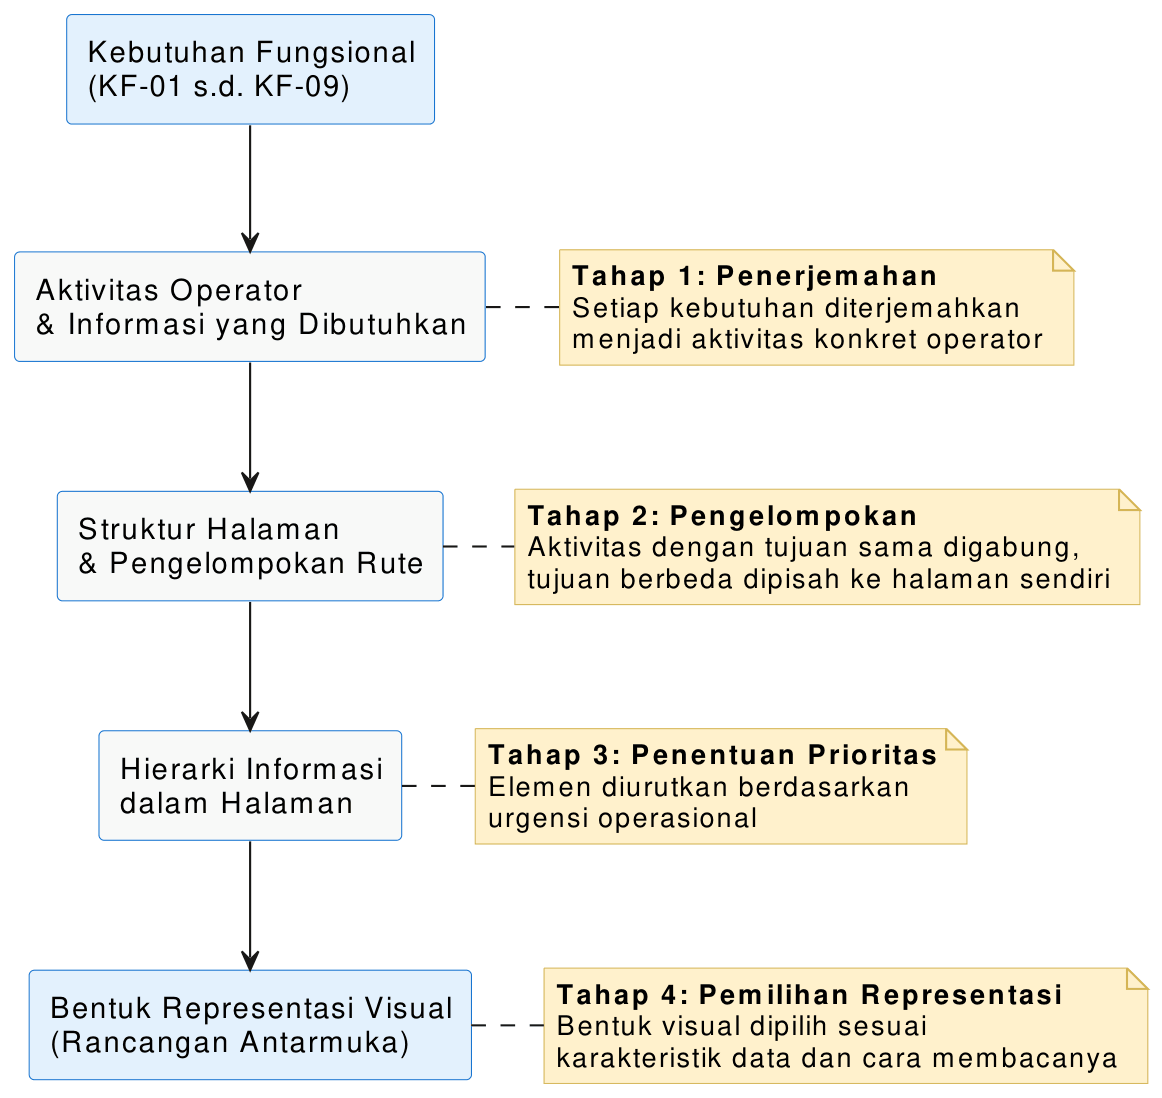
\includegraphics[width=0.7\textwidth]{images/tahapan-penurunan.png}
    \caption{Alur tahapan penurunan kebutuhan fungsional menjadi rancangan antarmuka}
    \label{fig:tahapan-penurunan}
\end{figure}

\begin{enumerate}
    \item \textbf{Penerjemahan kebutuhan menjadi aktivitas operator.} Setiap kebutuhan fungsional diterjemahkan 
    menjadi aktivitas konkret yang dilakukan operator beserta informasi yang dibutuhkan untuk menyelesaikan 
    aktivitas tersebut.
    
    \item \textbf{Pengelompokan aktivitas menjadi halaman.} Aktivitas dikelompokkan berdasarkan kesamaan tujuan 
    operasional. Aktivitas dengan tujuan berbeda dipisahkan ke halaman tersendiri sesuai prinsip kedua.
    
    \item \textbf{Penentuan hierarki informasi dalam halaman.} Pada setiap halaman, elemen informasi diurutkan 
    berdasarkan urgensi operasionalnya, yaitu seberapa cepat informasi tersebut dibutuhkan untuk mengenali kondisi 
    yang memerlukan tindakan. 
    
    \item \textbf{Pemilihan bentuk representasi visual.} Setiap elemen informasi dipetakan ke bentuk visualisasi 
    yang sesuai dengan karakteristik datanya dan dengan cara operator membacanya.
\end{enumerate}

Hasil penerapan keempat tahapan tersebut terhadap seluruh kebutuhan fungsional dirangkum pada 
Tabel~\ref{tab:penurunan-kf}.

\begin{table}[H]
\centering
\caption{Penurunan kebutuhan fungsional menjadi rancangan antarmuka}
\label{tab:penurunan-kf}
\renewcommand{\arraystretch}{1.25}
\small
\begin{tabular}{|c|p{3.2cm}|p{3.7cm}|p{2cm}|p{3.7cm}|}
\hline
\textbf{KF} & \textbf{Aktivitas Operator} & \textbf{Informasi Dibutuhkan} & \textbf{Halaman} & \textbf{Representasi} \\ \hline
KF-01 & Masuk dan keluar sistem & Kredensial dan status sesi & \texttt{/login} & Formulir autentikasi terisolasi \\ \hline
KF-02 & Menilai kondisi kualitas air secara sekilas & Nilai pH, kekeruhan, TDS, dan status kepatuhannya & \texttt{/dashboard} & Panel kepatuhan agregat dan kartu indikator per parameter \\ \hline
KF-03 & Memeriksa ketersediaan bahan kimia dan aktivitas pompa & Persentase dan volume tangki, status pompa & \texttt{/dashboard} & Indikator tangki analog serta penanda status pompa \\ \hline
KF-04 & Memastikan data yang dilihat masih valid & Waktu pembaruan terakhir dan status ketersediaan data & Seluruh halaman & Penanda waktu pembaruan dan lapisan peringatan \\ \hline
KF-05 & Menganalisis perilaku satu parameter secara mendalam & Nilai terkini, rentang target, statistik, dan tren & \texttt{/sensors} & Panel metrik dan grafik tren per parameter \\ \hline
KF-06 & Menelusuri riwayat dan menyusun laporan & Data historis pada rentang waktu tertentu & \texttt{/history} & Penyaring waktu, grafik, tabel audit, dan tombol ekspor \\ \hline
KF-07 & Menindaklanjuti kondisi anomali & Daftar alarm, tingkat keparahan, dan status penanganan & \texttt{/alarms} & Daftar vertikal dengan lencana dan tombol aksi \\ \hline
KF-08 & Mengoreksi dosis bahan kimia & Dosis terhitung dan \textit{offset} yang berlaku & \texttt{/pump-offset} & Kartu kendali per pompa dengan formulir masukan \\ \hline
KF-09 & Berpindah antaraktivitas pemantauan & Struktur navigasi aplikasi & Seluruh halaman & Panel navigasi persisten \\ \hline
\end{tabular}
\end{table}

\begin{figure}[H]
    \centering
    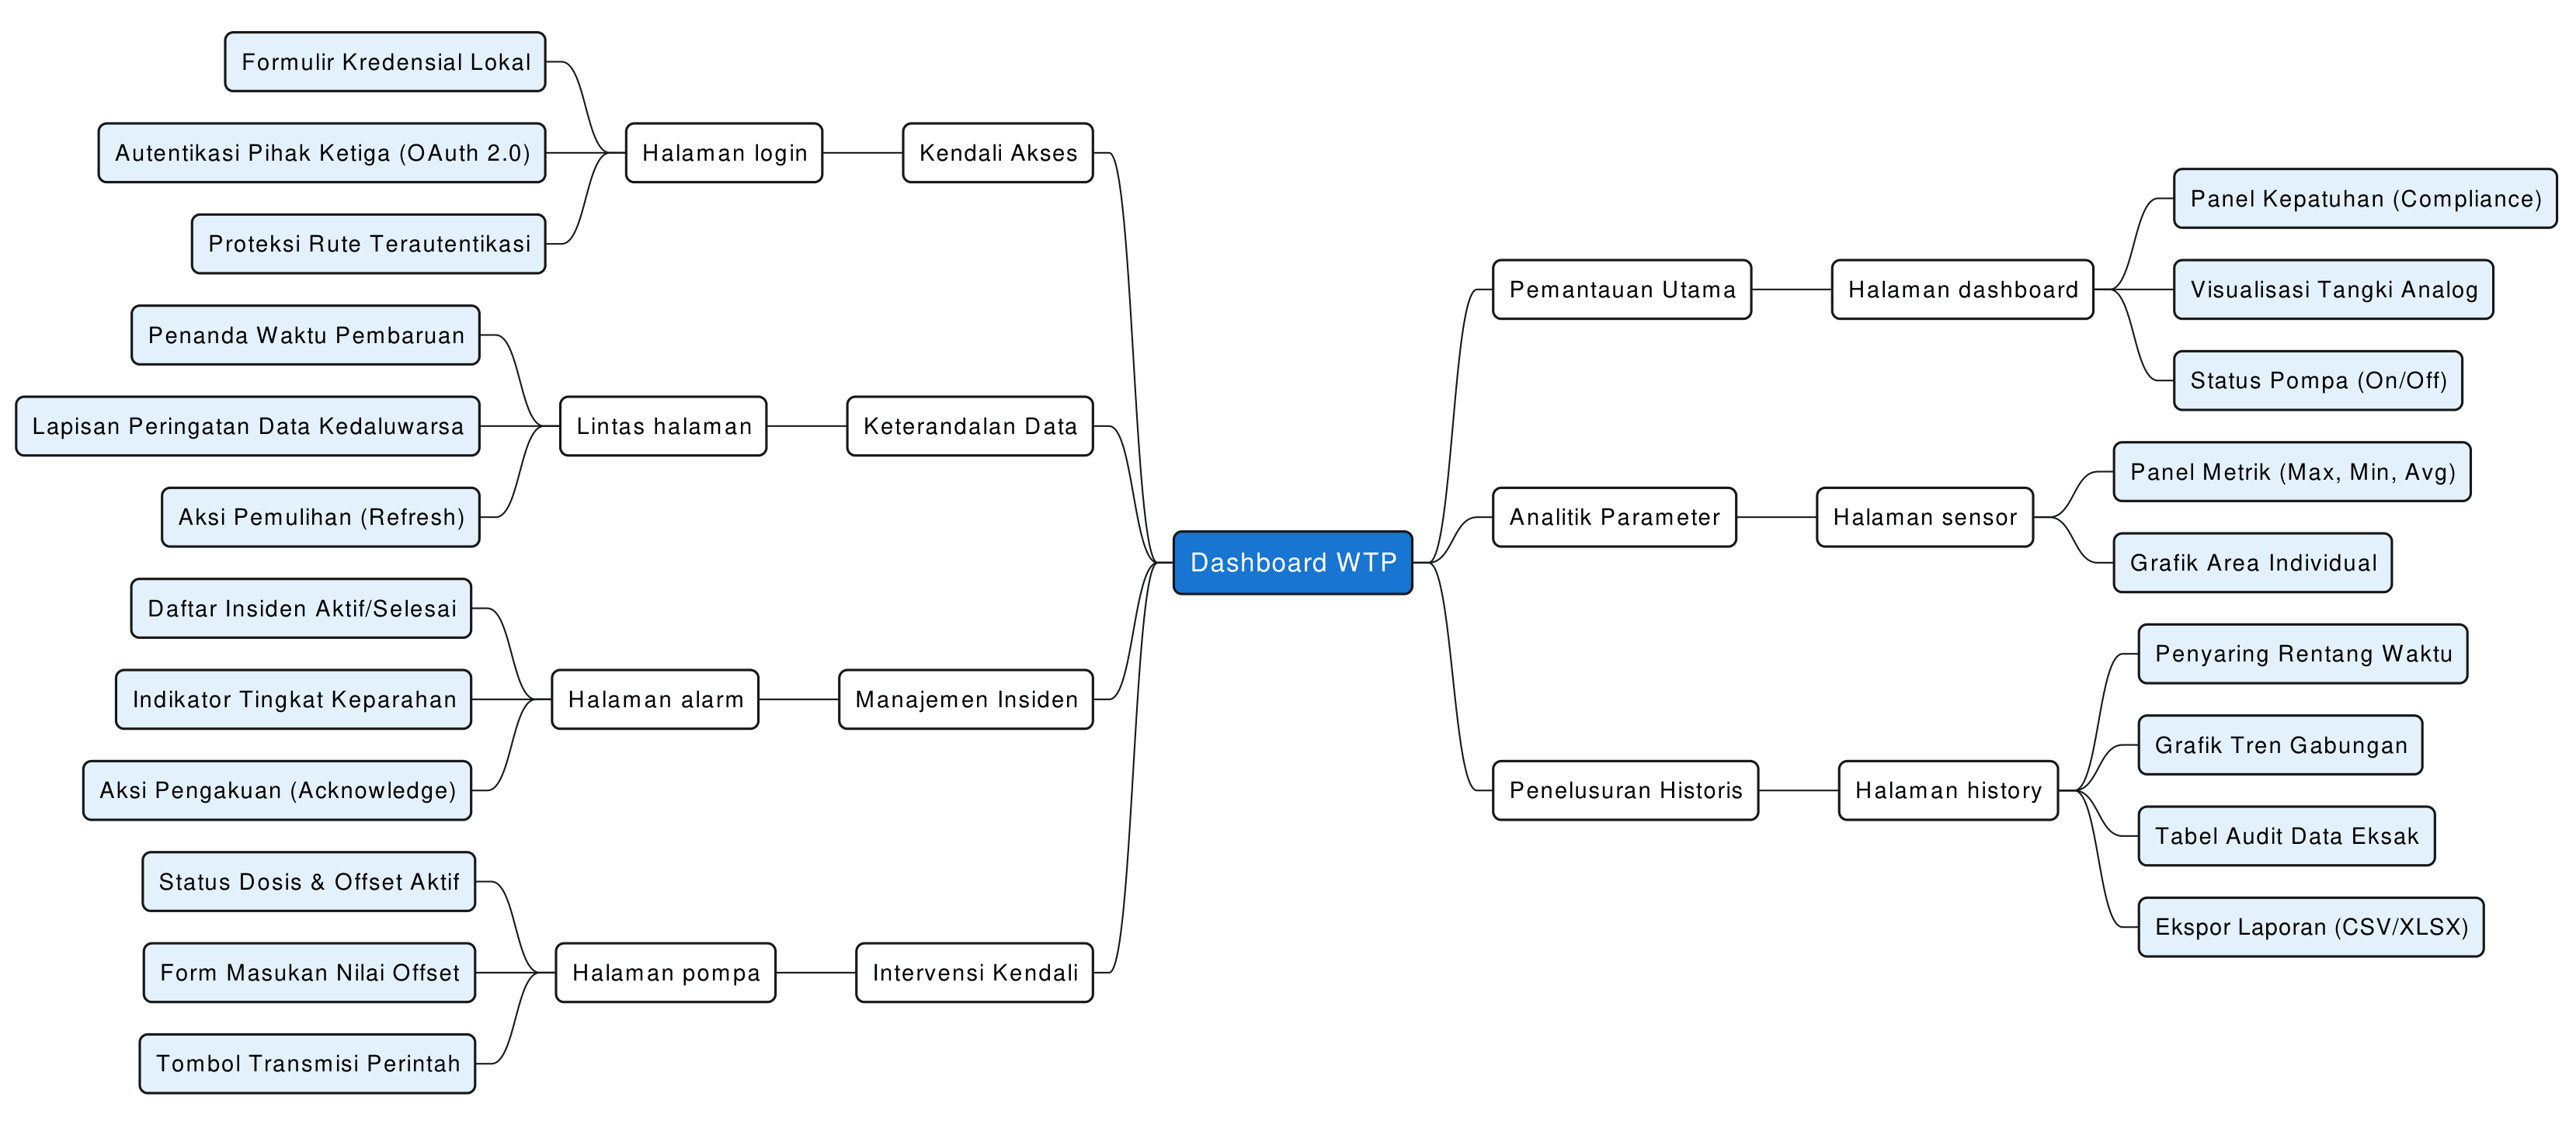
\includegraphics[width=\textwidth]{images/mindmap-dashboard.png}
    \caption{Peta hasil pemetaan kebutuhan fungsional menjadi struktur halaman dan komponen antarmuka}
    \label{fig:mindmap-dashboard}
\end{figure}

\subsection{Penurunan Rancangan Halaman \textit{Dashboard} Utama}
Sebagai penerapan tahapan di atas, berikut dijabarkan proses penurunan rancangan halaman 
\texttt{/dashboard}. Berdasarkan Tabel~\ref{tab:penurunan-kf}, halaman ini merealisasikan tiga kebutuhan 
sekaligus, yaitu KF-02, KF-03, dan KF-04.

\subsubsection{Penentuan Hierarki Informasi}
Ketiga kebutuhan tersebut diurutkan berdasarkan urgensi operasionalnya. KF-04 ditempatkan pada prioritas 
tertinggi karena seluruh informasi lain kehilangan maknanya apabila data yang ditampilkan ternyata sudah 
kedaluwarsa. Oleh sebab itu, penanda waktu pembaruan diletakkan berdampingan dengan panel kepatuhan, sedangkan 
peringatan data kedaluwarsa dirancang sebagai lapisan yang mengambil alih perhatian operator ketika kondisi 
tidak normal terjadi.

Prioritas berikutnya adalah KF-02, yaitu status kualitas air. Informasi ini menjawab pertanyaan pertama yang 
diajukan operator ketika membuka \textit{dashboard}, yaitu apakah kondisi instalasi sedang normal atau 
memerlukan tindakan. Karena bersifat menentukan tindakan lanjutan, komponen ini ditempatkan pada wilayah pandang 
utama, yaitu bagian teratas area konten.

Prioritas terakhir diberikan kepada KF-03, yaitu ketersediaan bahan kimia. Informasi ini bersifat penunjang 
karena berkaitan dengan perencanaan pengisian ulang, bukan dengan respons segera terhadap perubahan kualitas 
air. Oleh karena itu, komponen tersebut ditempatkan pada bagian bawah halaman.

\subsubsection{Iterasi Rancangan Panel Kepatuhan}
Rancangan awal halaman \textit{dashboard} memisahkan penyajian informasi ke dalam dua bagian, yaitu panel 
kepatuhan yang menyatakan pemenuhan parameter terhadap standar Permenkes dan bagian tersendiri yang menampilkan 
nilai pembacaan pH, kekeruhan, serta TDS. Setelah ditinjau kembali, rancangan tersebut dinilai menimbulkan dua 
persoalan. Pertama, nilai parameter kualitas air ditampilkan dua kali, yaitu sebagai dasar penilaian kepatuhan 
dan sebagai bagian tersendirisehingga terjadi redundansi informasi. Kedua, pemisahan tersebut memperpanjang 
halaman sehingga operator perlu menggulir layar untuk memperoleh gambaran kondisi secara utuh, yang bertentangan 
dengan prinsip minimalisasi perpindahan konteks.

Berdasarkan pertimbangan tersebut, tim memutuskan untuk menggabungkan kedua bagian menjadi satu komponen 
kepatuhan terpadu. Pada rancangan final, panel kepatuhan menyajikan status agregat (jumlah parameter yang berada 
dalam batas aman terhadap total parameter beserta persentasenya) dan sekaligus memuat kartu indikator untuk 
setiap parameter kualitas air maupun level tangki bahan kimia. Dengan demikian, satu komponen menjawab dua 
tingkat pertanyaan operator sekaligus, yaitu apakah kondisi instalasi secara keseluruhan aman, dan apabila tidak, 
parameter mana yang menyimpang.

\subsubsection{Pemilihan Bentuk Representasi Visual}
Pemilihan bentuk visual pada halaman ini didasarkan pada karakteristik data dan cara operator membacanya, 
sebagaimana dijabarkan berikut.

\begin{itemize}
    \item \textbf{Status kepatuhan} disajikan sebagai rasio dan persentase agregat karena operator membutuhkan 
    satu nilai tunggal yang dapat dinilai secara instan, bukan pembacaan berurutan atas seluruh parameter.
    
    \item \textbf{Nilai parameter kualitas air} disajikan sebagai kartu indikator dengan penanda warna. Bentuk 
    kartu dipilih karena setiap parameter merupakan nilai tunggal yang berdiri sendiri, sedangkan penanda warna 
    memungkinkan operator mengenali parameter yang menyimpang tanpa perlu membandingkan angka dengan batas 
    ambangnya secara manual.
    
    \item \textbf{Level tangki bahan kimia} disajikan melalui representasi analog berupa tabung terisi yang 
    dilengkapi nilai persentase dan volume tersedia. Representasi analog dipilih karena besaran proporsional 
    dapat dinilai lebih cepat secara visual dibandingkan pembacaan angka, sementara nilai numerik tetap 
    disertakan untuk keperluan presisi, misalnya ketika operator perlu memperkirakan waktu pengisian ulang. 
    Dengan demikian, representasi visual berperan untuk kecepatan penilaian, sedangkan nilai numerik berperan 
    untuk ketepatan.
    
    \item \textbf{Status pompa dosis} disajikan sebagai penanda ringkas karena hanya memiliki dua kemungkinan 
    keadaansehingga tidak memerlukan visualisasi yang kompleks.
\end{itemize}

Penurunan dengan tahapan yang sama diterapkan pada halaman-halaman lain, yang hasil rancangannya dijabarkan pada 
subbab berikutnya.
\section{Perancangan Arsitektur dan Interaksi Pengguna}
Bagian ini menjabarkan perancangan sistem pada tingkat abstraksi tertinggi, yang mencakup bagaimana pengguna berinteraksi 
dengan fungsionalitas sistem melalui pemodelan \textit{use case}, serta bagaimana data operasional mengalir dari perangkat keras 
di lapangan hingga disajikan ke layar \textit{dashboard} melalui arsitektur aliran data.

\subsection{Perancangan Interaksi Pengguna}
\label{subsec:use-case}
Interaksi fungsional antara pengguna dan \textit{frontend dashboard} WTP dimodelkan menggunakan \textit{Use Case Diagram}. 
Diagram ini mendefinisikan batasan sistem dan memetakan seluruh aktivitas operasional yang dapat dilakukan oleh aktor. 
Pada perancangan sistem kendali ini, satu-satunya aktor yang berinteraksi langsung dengan aplikasi adalah Operator WTP. 
Pemodelan \textit{use case} sistem ditunjukkan pada Gambar~\ref{fig:use-case}.

\begin{figure}[htbp]
    \centering
    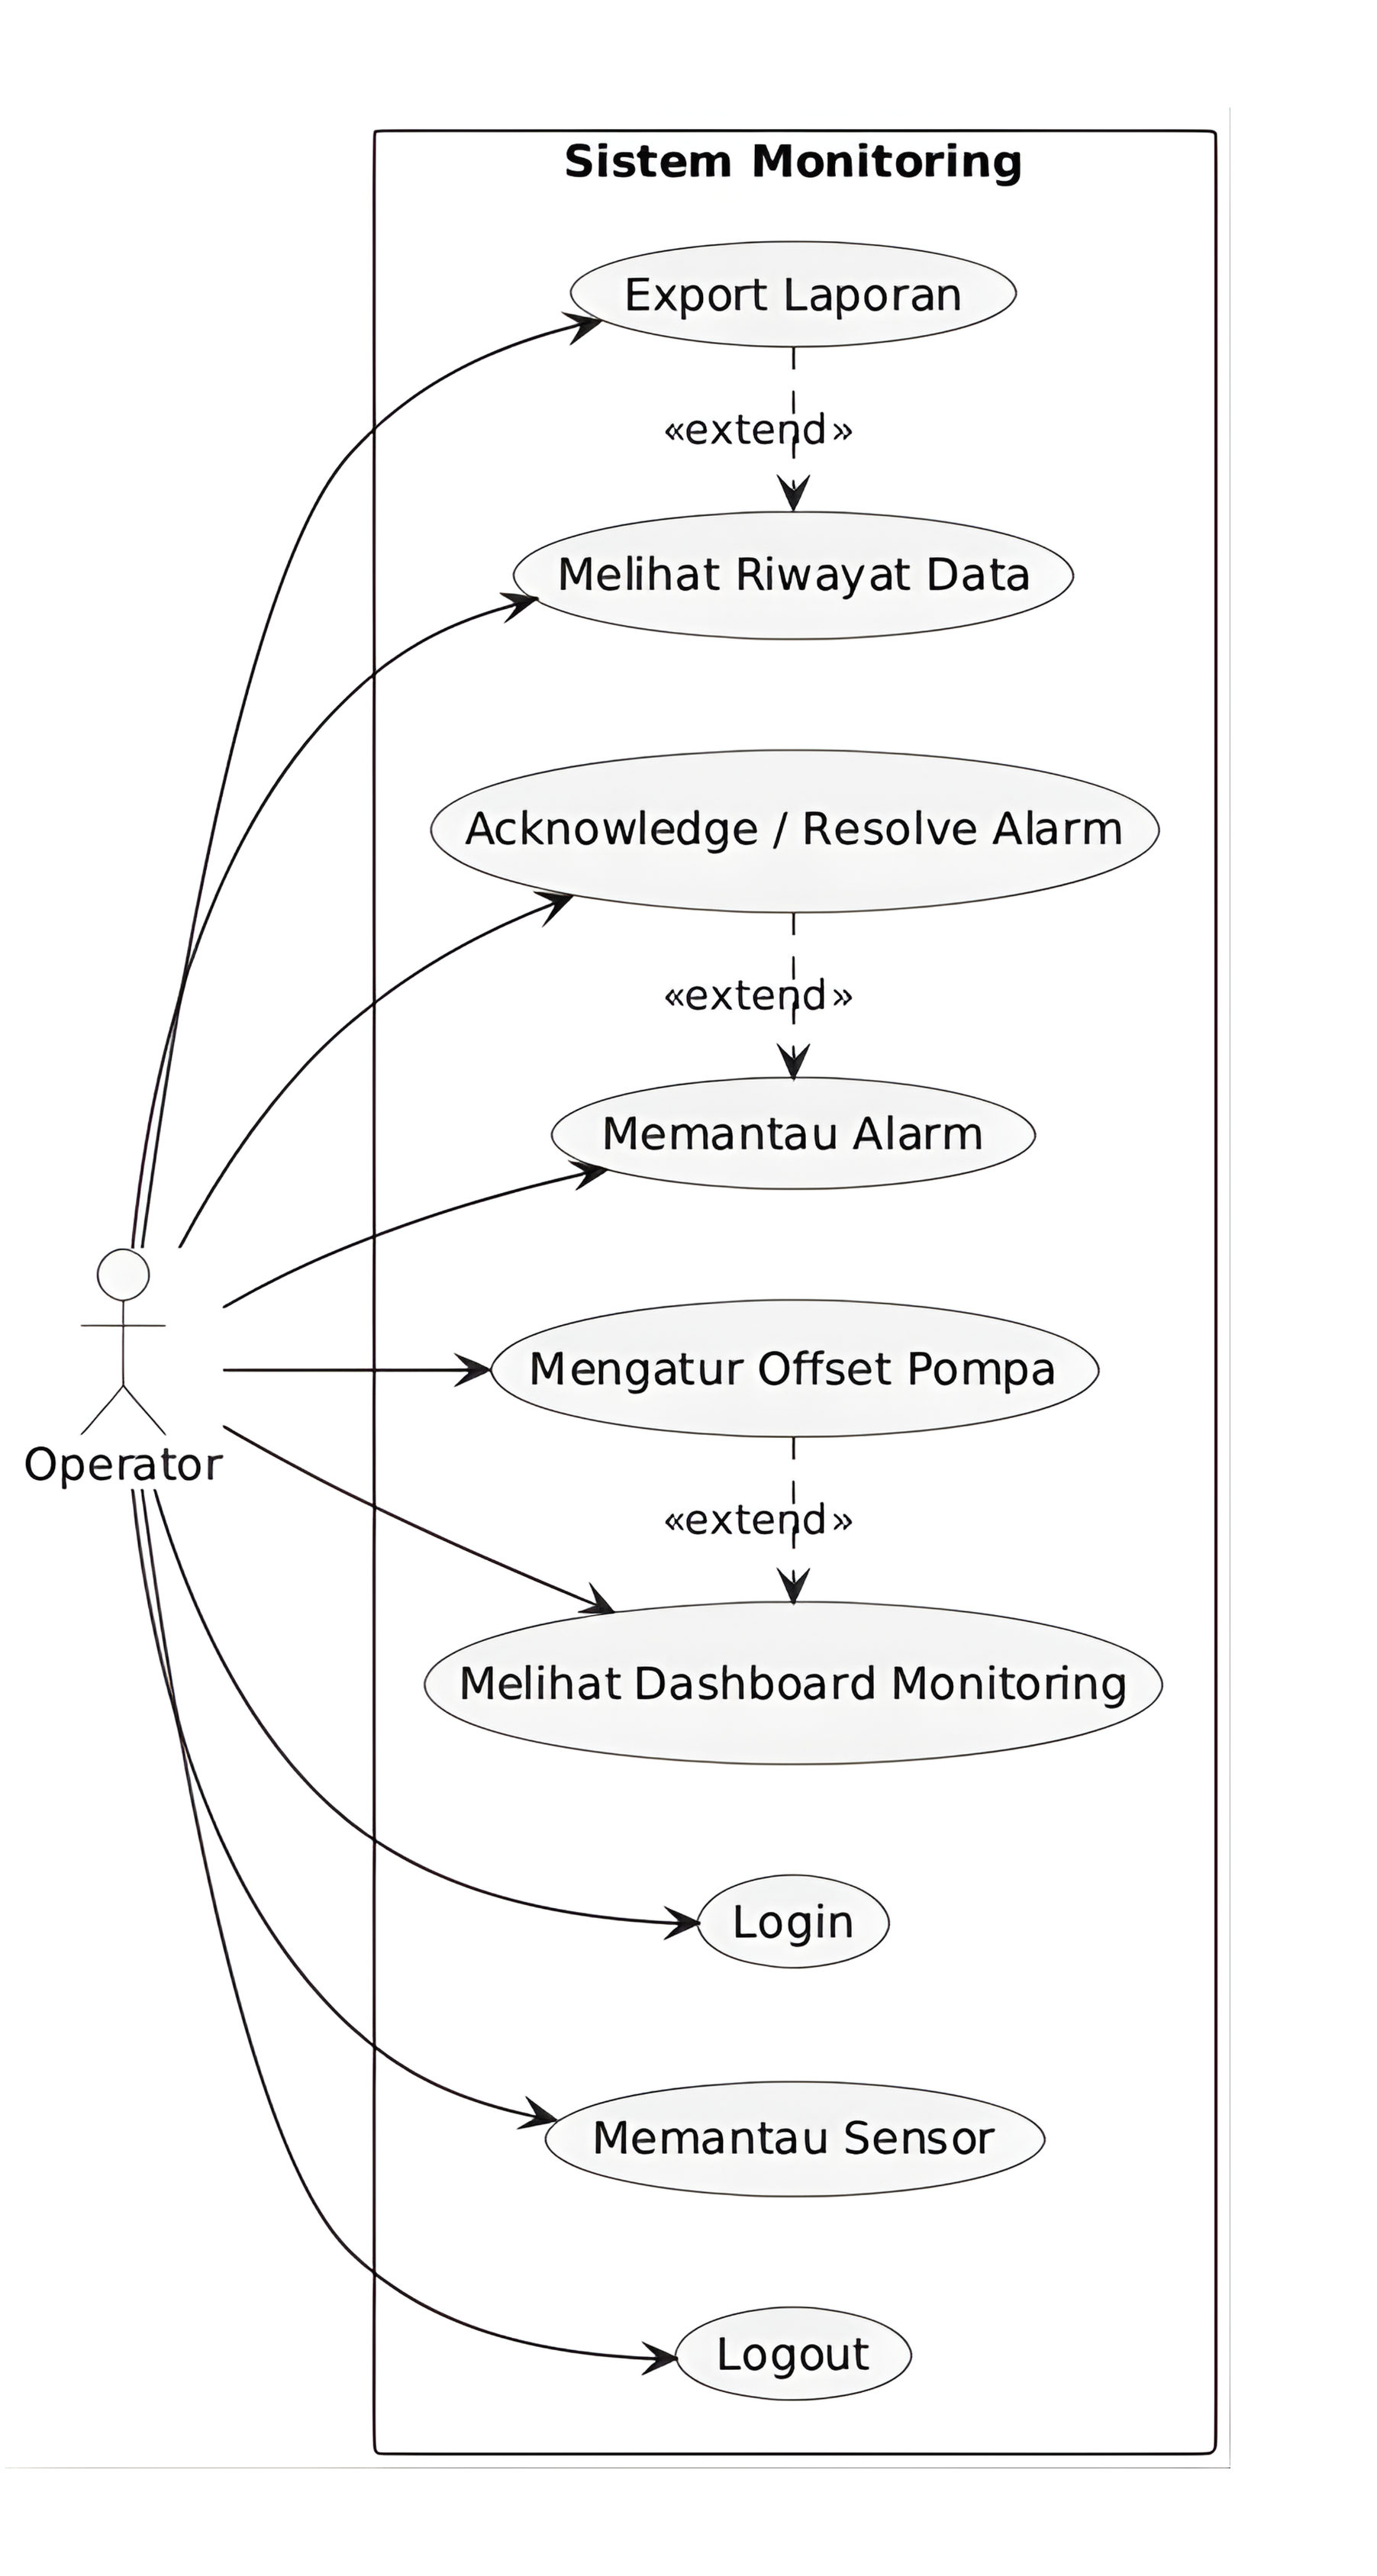
\includegraphics[width=0.7\textwidth]{images/finale.png}
    \caption{\textit{Use Case Diagram} sistem monitoring WTP}
    \label{fig:use-case}
\end{figure}

Berdasarkan Gambar~\ref{fig:use-case}, hak akses dan kapabilitas Operator direpresentasikan melalui serangkaian \textit{use case} utama 
dan \textit{use case} perluasan (\textit{extend}). Rincian fungsionalitas operasional tersebut adalah sebagai berikut:
\begin{itemize}
    \item \textbf{\textit{Login} dan \textit{Logout}:} Aktivitas fundamental untuk autentikasi sesi dan perlindungan rute. 
    Operator diwajibkan untuk masuk ke dalam sistem (\textit{login}) menggunakan kredensial yang sah sebelum dapat mengakses 
    fungsionalitas operasional. Sebaliknya, proses \textit{logout} digunakan untuk mematikan sesi dan mengamankan aplikasi saat 
    operator meninggalkan ruang kendali.
    \item \textbf{Memantau Sensor:} Fungsionalitas inti yang memfasilitasi operator untuk mengobservasi pembacaan instrumen 
    kualitas air, seperti metrik pH dan kekeruhan, secara \textit{real-time}.
    \item \textbf{Melihat \textit{Dashboard Monitoring}:} Aktivitas ini memberikan pandangan komprehensif 
    (\textit{helicopter view}) terhadap seluruh status WTP, termasuk level tangki bahan kimia dan status elektris pompa. 
    Fungsionalitas ini dapat diperluas (\textit{extend}) dengan \textbf{Mengatur \textit{Offset} Pompa}, yang memberikan 
    kewenangan bagi operator untuk mengintervensi otomasi dengan memberikan nilai kalibrasi atau penyesuaian dosis (\textit{offset}) 
    PAC dan kaporit langsung dari antarmuka \textit{dashboard}.
    \item \textbf{Memantau Alarm:} Modul bagi operator untuk mengawasi sistem peringatan dini manakala parameter telemetri menyimpang 
    dari ambang batas toleransi (\textit{threshold}). Aktivitas ini memiliki perluasan berupa 
    \textbf{\textit{Acknowledge} / \textit{Resolve} Alarm}, yang mewajibkan operator untuk memberikan konfirmasi visual bahwa suatu 
    insiden telah diketahui atau ditanganisehingga sistem dapat memperbarui status mitigasi alarm tersebut.
    \item \textbf{Melihat Riwayat Data:} Fasilitas analitik bagi operator untuk menelusuri data historis telemetri dan log sistem 
    berdasarkan penyaringan rentang waktu. Aktivitas ini diperluas dengan \textbf{\textit{Export} Laporan}, yang memungkinkan operator 
    mengunduh agregasi data ke dalam format berkas tabular (seperti CSV atau XLSX) untuk mendukung kebutuhan pelaporan teknis maupun 
    audit lingkungan.
\end{itemize}

\subsection{Perancangan Arsitektur Aliran Data}
Untuk mendukung interaksi fungsional yang telah didefinisikan pada \textit{use case}, dirancang sebuah arsitektur aliran data 
(\textit{data flow}) yang menjamin sinkronisasi informasi secara efisien. Perancangan ini memetakan perjalanan data mentah mulai 
dari lapisan perangkat keras hingga dirender menjadi elemen antarmuka yang interaktif di \textit{frontend}. Pemodelan aliran data 
tersebut diilustrasikan pada Gambar~\ref{fig:flow-data}.

\begin{figure}[htbp]
    \centering
    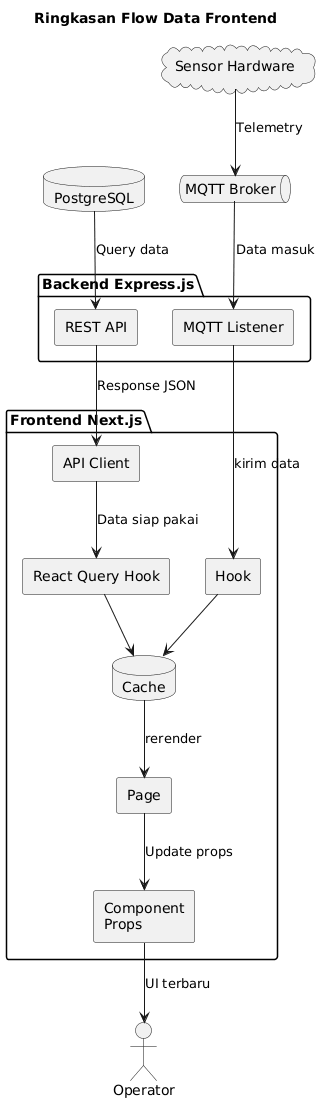
\includegraphics[height=0.8\textheight]{images/dataflow.png}
    \caption{Arsitektur aliran data (\textit{flow data}) pada \textit{frontend}}
    \label{fig:flow-data}
\end{figure}

Arsitektur pada Gambar~\ref{fig:flow-data} merepresentasikan pemisahan tanggung jawab (\textit{separation of concerns}) 
di berbagai lapisan sistem. Rincian aliran data dari hulu ke hilir adalah sebagai berikut:
\begin{enumerate}
    \item \textbf{Lapisan Akuisisi (\textit{Hardware Layer}):} \textit{Sensor Hardware} yang dipasang pada infrastruktur WTP 
    bertugas membaca parameter fisis dan menerjemahkannya menjadi data telemetri. Data tersebut dipublikasikan secara berkala 
    menuju \textit{Broker} Pesan menggunakan protokol komunikasi yang ringan dan tahan terhadap latensi jaringan.
    \item \textbf{Lapisan Layanan (\textit{Backend Layer}):} Layanan \textit{backend} mengadopsi 
    dua strategi penerimaan data. Pertama, modul penangkap pesan (\textit{listener}) berlangganan (\textit{subscribe}) ke topik \textit{broker} 
    untuk menangkap aliran data masuk (\textit{data stream}). Kedua, sistem mengeksekusi kueri ke Sistem Manajemen Basis Data (DBMS) relasional untuk menarik 
    data historis. Hasil pemrosesan dari kedua sumber tersebut dibungkus oleh antarmuka pemrograman aplikasi (\textit{REST API}) ke dalam format respons pertukaran data standar.
    \item \textbf{Lapisan Klien (\textit{Frontend Layer}):} Aplikasi klien (\textit{frontend}) 
    mengkonsumsi data dari layanan \textit{backend}. Modul klien API memfasilitasi pengambilan data secara asinkron. 
    Data yang telah siap pakai kemudian diserahkan kepada modul manajemen \textit{state} asinkron. Di sisi lain, 
    pembaruan data kejadian \textit{real-time} (seperti pemicuan alarm) dapat ditangkap oleh modul reaktif lainnya untuk diteruskan 
    ke dalam memori lokal aplikasi.
    \item \textbf{Mekanisme \textit{Caching} dan Perenderan UI:} Seluruh data yang berhasil ditarik akan diinjeksi ke dalam memori 
    sementara (\textit{Cache}). Pendekatan ini mencegah aplikasi melakukan permintaan jaringan (\textit{network request}) yang redundan. 
    Ketika terjadi pembaruan data di dalam \textit{Cache}, komponen halaman (\textit{Page}) akan bereaksi dengan mendistribusikan data 
    terbaru tersebut sebagai properti turunan (\textit{Component Props}). Transmisi properti ini memicu proses perenderan ulang (\textit{rerender}) 
    pada komponen antarmuka sehingga UI terbaru dapat segera direfleksikan di layar Operator dengan performa yang optimal.
\end{enumerate}

\section{Perancangan Struktur Halaman dan Routing}
\label{subsec:routing}
Perancangan struktur halaman dan \textit{routing} pada aplikasi \textit{dashboard} WTP dikembangkan menggunakan 
arsitektur \textit{Single Page Application} (SPA), yang memungkinkan perpindahan antarmuka terjadi secara instan 
tanpa memuat ulang seluruh halaman peramban.

Berbeda dengan aplikasi web pada umumnya yang menyediakan beberapa rute publik (misalnya pendaftaran akun, 
pemulihan kata sandi, atau laman informasi umum), sistem ini dirancang dengan hanya satu rute publik, yaitu 
\texttt{/login}. Keputusan ini diambil karena operator WTP merupakan pengguna internal yang akun aksesnya 
didaftarkan langsung oleh admin, bukan melalui pendaftaran mandiri. Dengan demikian, seluruh 
fungsionalitas lain dari sistem, tanpa kecuali, berada di dalam wilayah rute terproteksi.

Proteksi rute diimplementasikan pada satu titik terpusat, yaitu \textit{middleware} yang membungkus seluruh 
halaman operasional, bukan pada tingkat masing-masing komponen halaman. Keputusan arsitektural ini memastikan 
setiap rute baru yang ditambahkan di kemudian hari akan otomatis mewarisi mekanisme proteksi tanpa memerlukan 
implementasi pengecekan sesi secara berulang pada setiap halaman.

Rute \texttt{/login} sendiri dilengkapi dengan logika pencegatan (\textit{interceptor}): apabila pengguna yang 
sudah memiliki sesi aktif mencoba mengakses rute ini, sistem secara otomatis mengalihkannya ke halaman 
\textit{dashboard}. Keputusan ini diambil untuk mencegah kebingungan operator yang secara tidak sengaja kembali 
ke halaman login (misalnya melalui tombol kembali pada peramban) padahal sesinya masih berlaku.

Alur validasi token sesi dan penentuan akses ditunjukkan pada Gambar~\ref{fig:flowchart-routing}.

\begin{figure}[htbp]
    \centering
    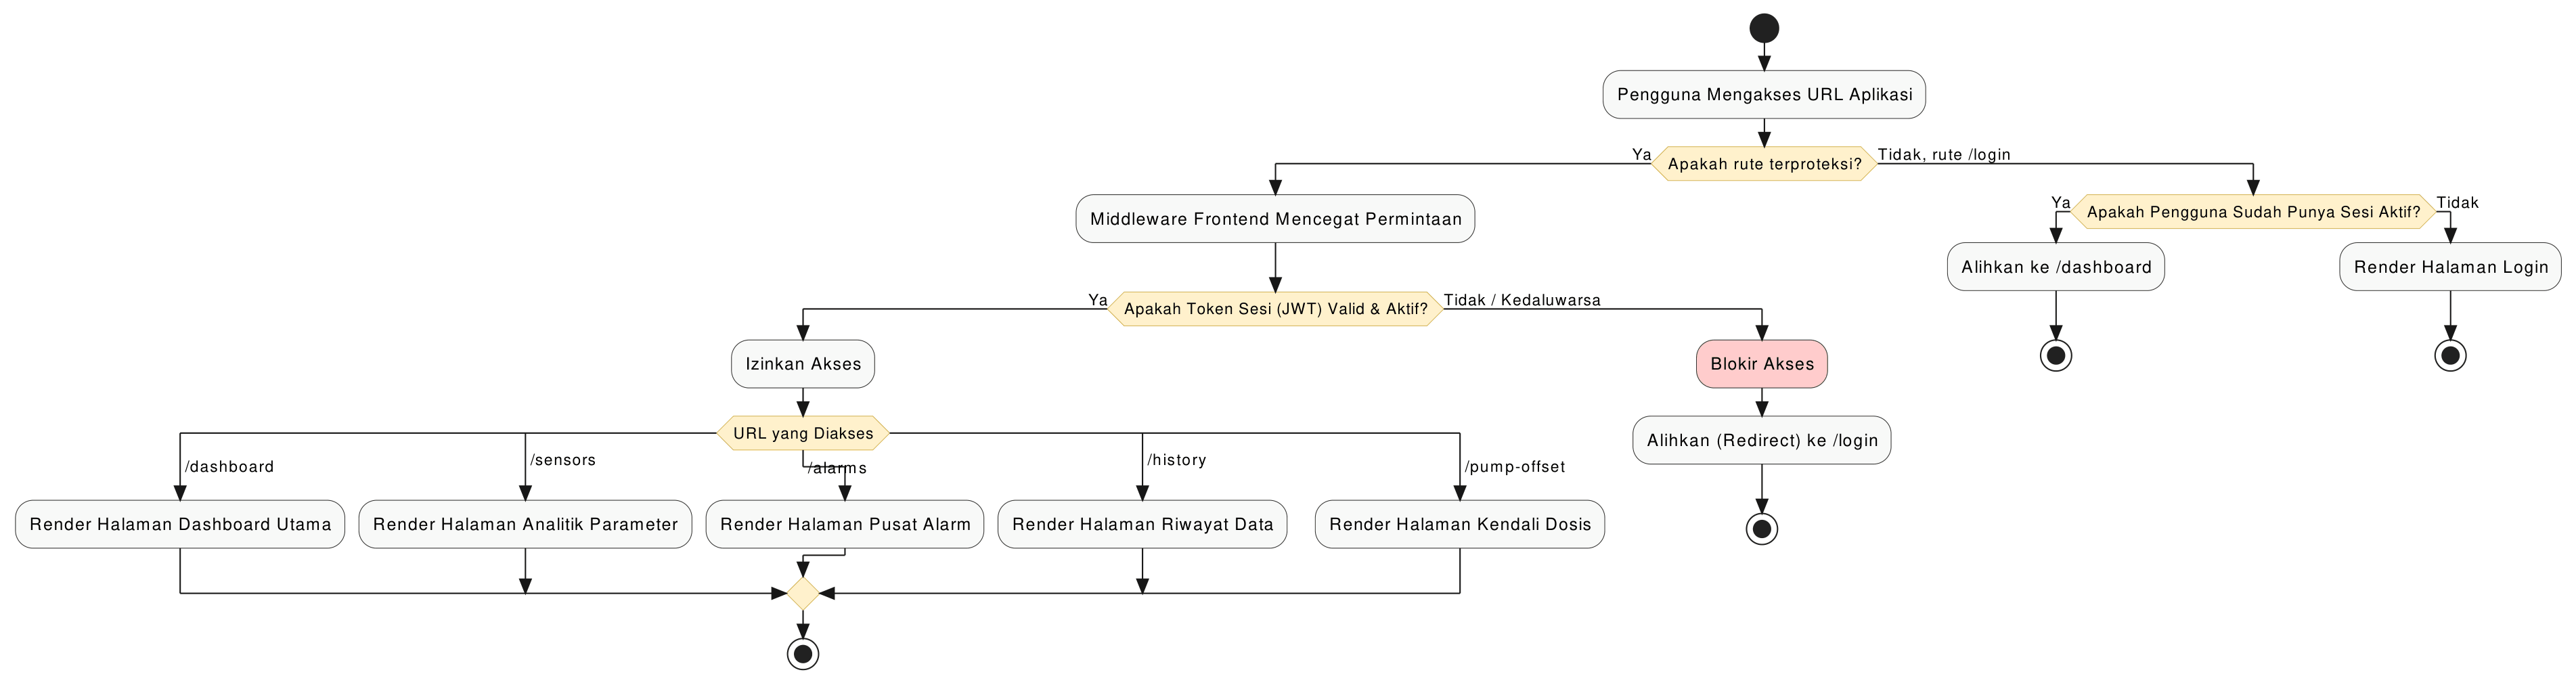
\includegraphics[width=1.15\textwidth]{images/flowchart-routing.png}
    \caption{Alur validasi sesi dan penentuan akses rute}
    \label{fig:flowchart-routing}
\end{figure}

\subsection{Rute Publik (\textit{Public Route})}
Rute publik mendefinisikan sekumpulan halaman yang bertindak sebagai pintu gerbang sistem dan dapat diakses oleh siapa saja 
tanpa memerlukan token autentikasi. Namun, untuk mengoptimalkan pengalaman pengguna (\textit{User Experience}), rute ini dilengkapi 
dengan logika pencegatan (\textit{interceptor}). Apabila pengguna yang sudah memiliki sesi aktif (\textit{logged in}) mencoba mengakses 
rute ini, sistem akan secara otomatis mengalihkannya (\textit{redirect}) ke halaman utama \textit{dashboard}.
\begin{itemize}
    \item \texttt{/login}: Merupakan antarmuka fundamental untuk proses autentikasi. Halaman ini menyajikan formulir bagi 
    operator untuk memasukkan kredensial (\textit{username} dan \textit{password}). Desain antarmuka dibuat terisolasi dan 
    minimalis agar operator dapat berfokus pada proses validasi keamanan.
\end{itemize}

\subsection{Rute Terproteksi (\textit{Protected Route})}
Rute terproteksi adalah wilayah sistem yang menyimpan seluruh data rahasia dan fungsionalitas kritis operasional WTP. 
Akses menuju seluruh halaman di dalam rute ini dijaga secara ketat oleh perantara (\textit{middleware}) autentikasi di sisi klien. 
Setiap kali pengguna melakukan navigasi ke rute ini, sistem akan memvalidasi keberadaan dan masa berlaku token sesi. Jika 
token tidak valid atau kedaluwarsa, akses akan ditolak dan pengguna dikembalikan secara paksa ke halaman \texttt{/login}.
\begin{itemize}
    \item \texttt{/dashboard}: Berfungsi sebagai pusat komando utama (\textit{at-a-glance monitoring}). 
    Halaman ini menyajikan panel kepatuhan instalasi (\textit{plant compliance}) yang menampilkan jumlah parameter 
    berada dalam rentang aman beserta persentase kepatuhannya, deretan kartu indikator untuk parameter kualitas air 
    (pH, kekeruhan, TDS) dan level bahan kimia (kaporit, PAC, soda ash), penanda waktu pembaruan terakhir data sensor 
    maupun tangki, serta visualisasi level tangki penyimpanan bahan kimia lengkap dengan volume tersedia dan indikator 
    status ketersediaannya.
    
    \item \texttt{/sensors}: Modul analitik per parameter. Halaman ini menyajikan setiap parameter kualitas air 
    (pH, kekeruhan, dan TDS) dalam bagian yang terpisah. Pada setiap bagian, sisi kiri memuat panel metrik berisi 
    nilai terkini, rentang target parameter, serta ringkasan statistik harian (nilai maksimum, minimum, dan rata-rata), 
    sedangkan sisi kanan memuat kanvas grafik tren yang menggambarkan perubahan parameter tersebut terhadap waktu.
    
    \item \texttt{/history}: Modul peninjauan dan pelaporan historis. Halaman ini menyediakan penyaring rentang waktu 
    yang dapat ditentukan secara manual melalui masukan periode awal dan periode akhir, maupun melalui rentang cepat 
    (\textit{quick range}) 24 jam, 7 hari, dan 30 hari. Data hasil penyaringan disajikan dalam dua bentuk yang saling 
    melengkapi, yaitu grafik tren gabungan ketiga parameter dan tabel audit telemetri yang memuat nilai eksak setiap 
    titik pengukuran. Halaman ini juga menyediakan fasilitas ekspor data ke dalam format berkas tabular (CSV atau XLSX) 
    untuk mendukung kebutuhan pelaporan teknis maupun audit lingkungan.
    
    \item \texttt{/alarms}: Halaman pemantauan anomali dan manajemen insiden. Bagian atas halaman menyajikan ringkasan 
    status alarm berupa jumlah alarm kritis dan tingkat penyelesaian (\textit{resolution rate}). Bagian utama halaman 
    memuat daftar kejadian (\textit{event log}) yang dapat dipilah melalui penyaring antara alarm aktif dan alarm 
    terselesaikan. Setiap baris kejadian menampilkan lencana tingkat keparahan, deskripsi anomali beserta nilai 
    pembacaan dan ambang batas yang terlampaui, cap waktu kejadian, serta tombol pengakuan (\textit{acknowledge}) 
    yang memungkinkan operator menindaklanjuti alarm secara langsung dari daftar tersebut.
    
    \item \texttt{/pump-offset}: Halaman intervensi dosis dengan tingkat sensitivitas tertinggi. Halaman ini menyajikan 
    kartu terpisah untuk setiap pompa injeksi bahan kimia, yaitu pompa \textit{Polyaluminium Chloride} (PAC), pompa 
    kaporit, dan pompa soda ash. Setiap kartu menampilkan nilai dosis hasil kalkulasi sistem dan nilai \textit{offset} 
    yang sedang aktif, serta menyediakan kolom masukan untuk menetapkan nilai \textit{offset} baru dalam satuan mililiter 
    beserta tombol eksekusi pengiriman. Nilai \textit{offset} yang diberikan bersifat sementara dan direset secara 
    otomatis setelah setiap sesi pemompaan berakhir.
\end{itemize}

\subsection{Alur Navigasi Pengguna}
Alur navigasi (\textit{user journey}) dirancang secara hierarkis dan linear untuk meminimalisasi kebingungan operator saat 
memantau kondisi WTP. Titik awal navigasi selalu bermula dari halaman \texttt{/login}. Setelah proses otorisasi berhasil 
divalidasi oleh layanan \textit{backend}, operator langsung diarahkan ke halaman \texttt{/dashboard}.

Dari halaman \texttt{/dashboard} tersebut, operator diberikan fleksibilitas untuk mengeksplorasi modul-modul turunan melalui 
bilah navigasi persisten (\textit{sidebar navigation}). Alur hierarki navigasi tersebut dapat dipetakan sebagai berikut:

\begin{itemize}
    \item \textbf{Autentikasi:} \texttt{/login} $\rightarrow$ \textit{Redirect} ke \textit{Dashboard}
    \item \textbf{Navigasi Utama (\textit{Dashboard}):} 
    \begin{itemize}
        \item Meninjau analitik terperinci per parameter (\texttt{/sensors})
        \item Menelusuri riwayat dan mengekspor laporan (\texttt{/history})
        \item Meninjau dan menindaklanjuti insiden (\texttt{/alarms})
        \item Melakukan intervensi otomasi bahan kimia (\texttt{/pump-offset})
    \end{itemize}
\end{itemize}

Pemisahan struktur halaman dan logika \textit{routing} ini memastikan bahwa arsitektur \textit{frontend} tidak hanya 
andal dalam menyajikan data operasional, tetapi juga kokoh dalam melindungi fungsionalitas sistem dari akses entitas yang tidak berwenang.

\section{Perancangan Antarmuka Pengguna}
\label{subsec:ui-design}
Antarmuka pengguna dirancang untuk menerjemahkan kompleksitas data telemetri dan operasional WTP menjadi representasi 
visual yang intuitif bagi operator. Proses perancangan diawali dengan pembuatan purwarupa tingkat rendah 
(\textit{low-fidelity wireframe}) untuk memetakan hierarki informasi dan tata letak (\textit{layout}) komponen 
fundamental sebelum memasuki tahap implementasi kode. Pendekatan ini bertujuan untuk memastikan alur navigasi dan 
penyajian data disusun berdasarkan prioritas keselamatan dan efisiensi operasional.

Seluruh antarmuka dikembangkan dengan prinsip desain responsif agar tetap proporsional ketika diakses melalui perangkat 
\textit{desktop} di ruang kendali maupun perangkat bergerak (\textit{mobile}) saat operator melakukan patroli lapangan. 

\subsection{Antarmuka Halaman \textit{Dashboard} Utama}
Halaman \textit{dashboard} bertindak sebagai pusat informasi sekilas (\textit{at-a-glance monitoring}). 
Tata letak dirancang untuk menonjolkan metrik paling kritis agar operator dapat mengenali status sistem dalam 
hitungan detik. Rancangan purwarupa halaman ini ditunjukkan pada Gambar~\ref{fig:ui-dashboard}.

\begin{figure}[htbp]
    \centering
    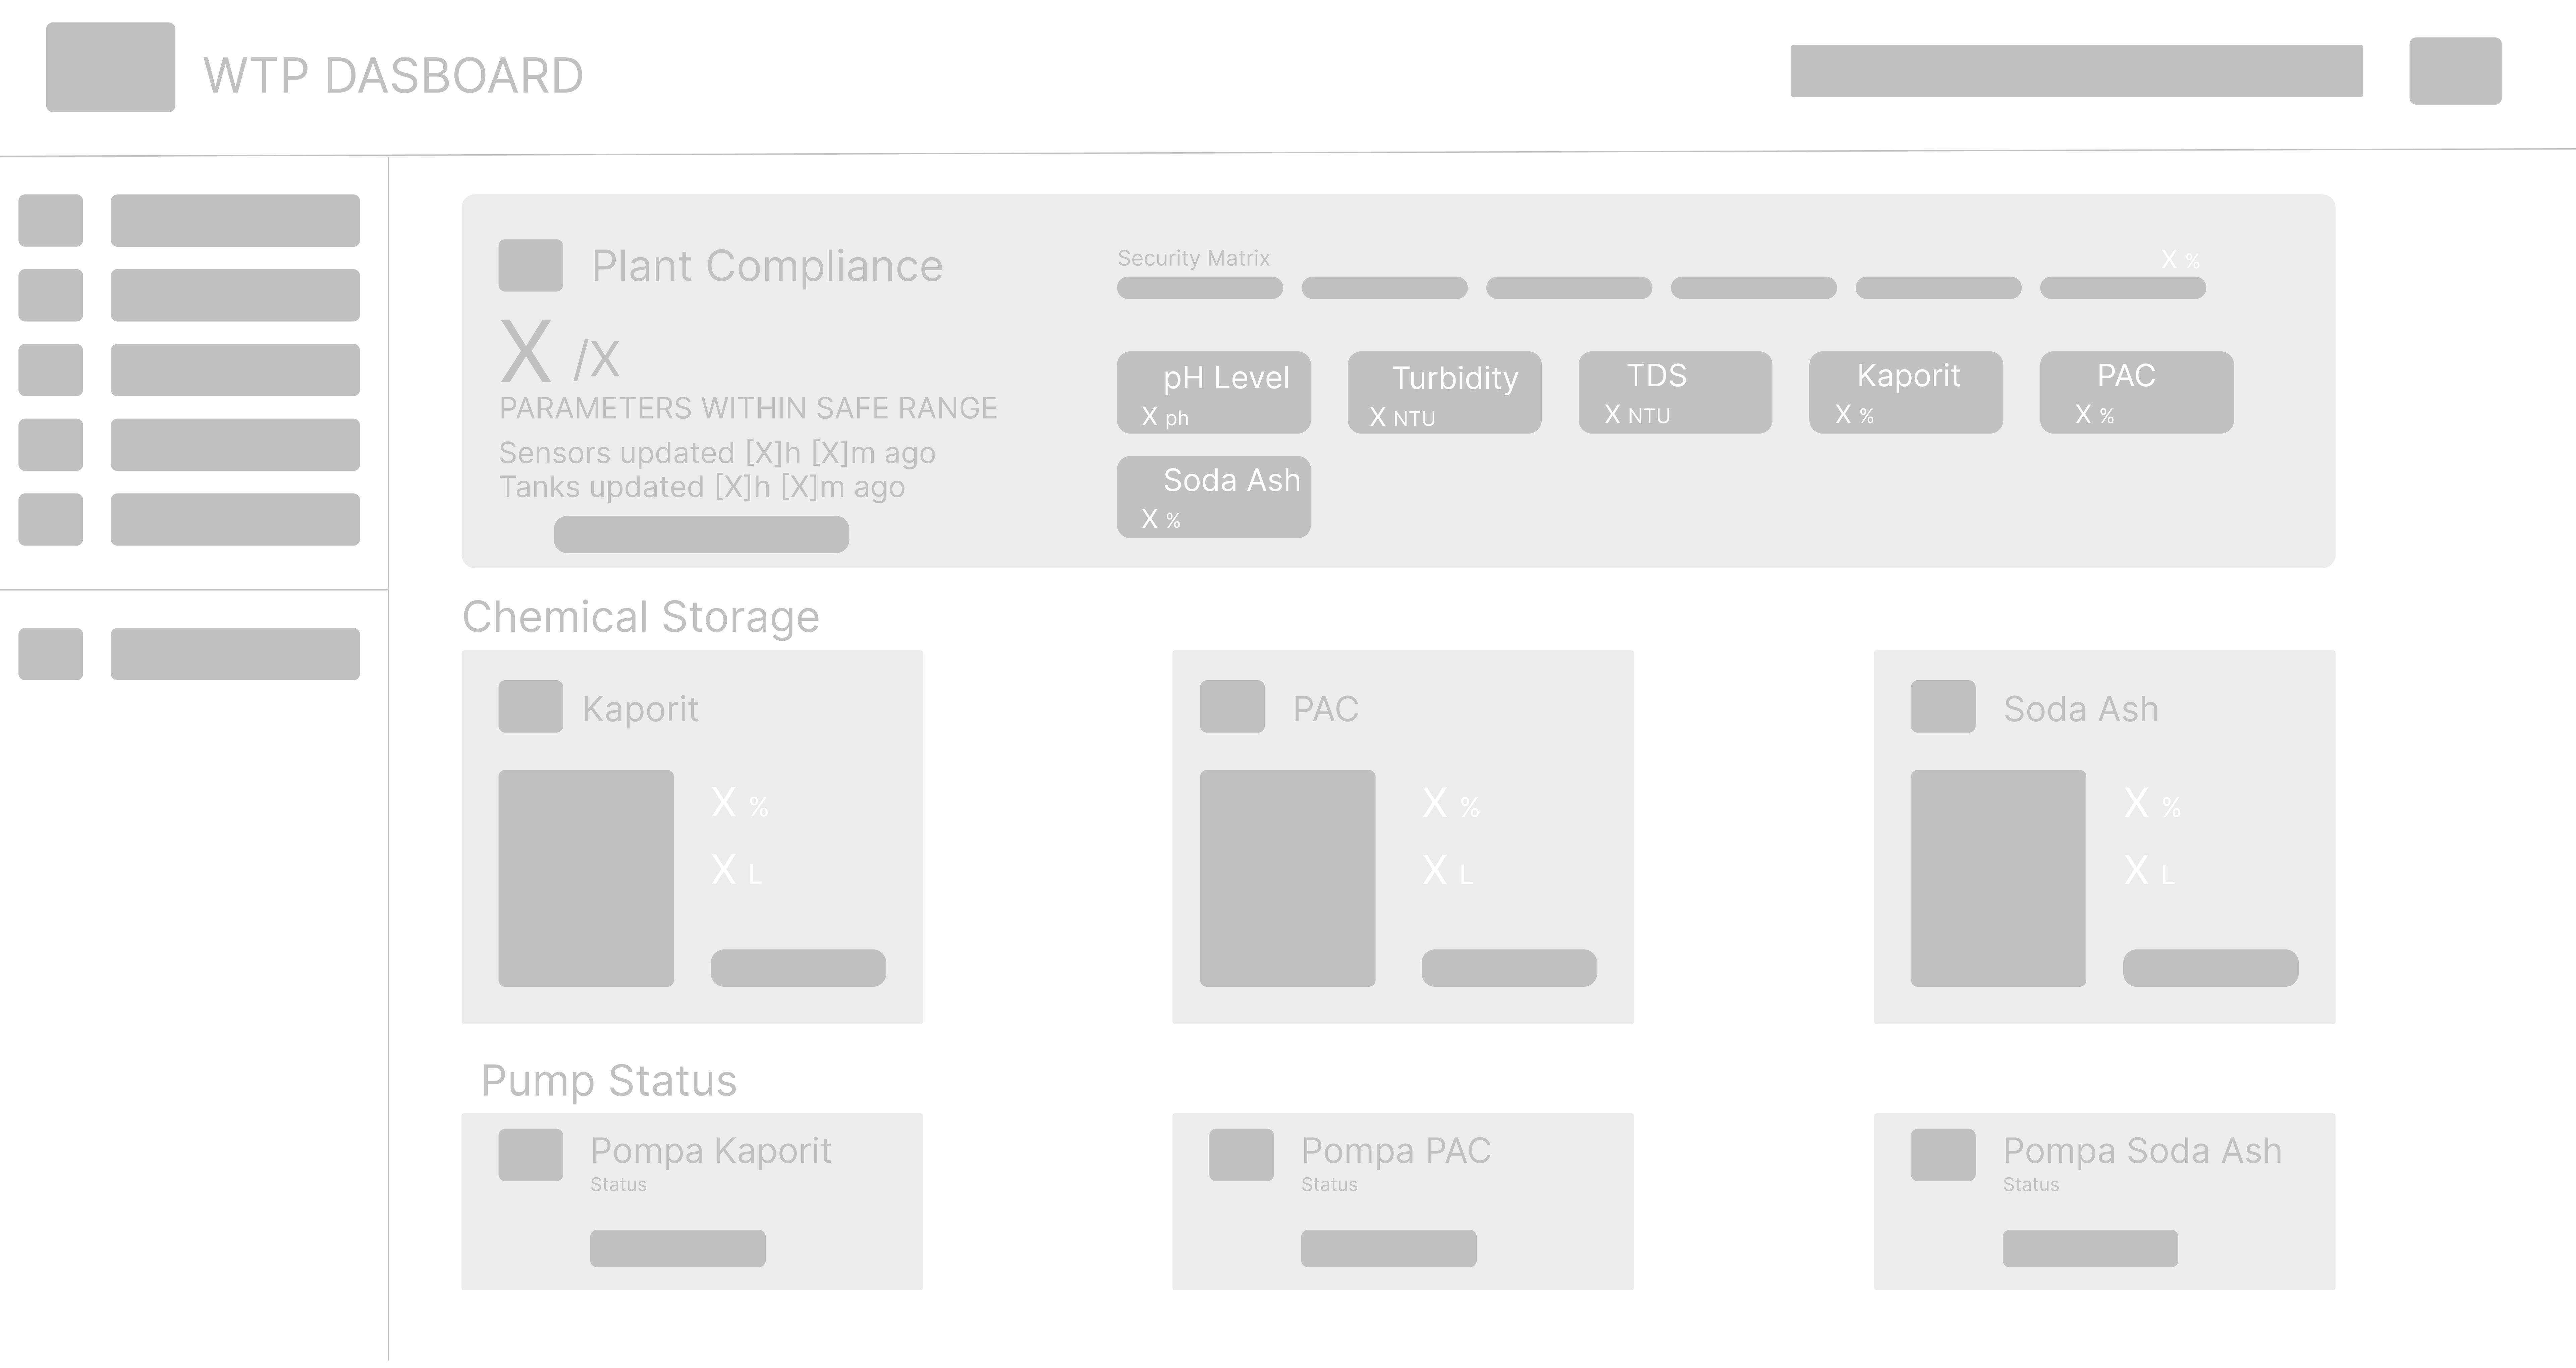
\includegraphics[width=\textwidth]{images/dash-lowfi.png}
    \caption{Rancangan purwarupa \textit{low-fidelity} halaman \textit{dashboard} utama}
    \label{fig:ui-dashboard}
\end{figure}

Berdasarkan Gambar~\ref{fig:ui-dashboard}, antarmuka dibagi menjadi dua area struktural. Sisi kiri dialokasikan untuk panel 
navigasi global (\textit{sidebar}) yang persisten, memudahkan perpindahan antarmodul tanpa kehilangan konteks. 
Pada area konten utama di sisi kanan, bagian teratas diisi dengan deretan kartu Indikator Kinerja Utama 
(\textit{Key Performance Indicator cards}). Penempatan komponen ini di bagian atas (wilayah pandang utama pengguna) 
bertujuan untuk menyorot nilai parameter esensial seperti pH, kekeruhan, serta level tangki secara instan. Area di bawahnya 
dikhususkan untuk visualisasi pendukung, seperti grafik sekilas dan status aktuator elektromekanis.

\subsection{Antarmuka Peringatan Data Kedaluwarsa}
\label{subsec:ui-stale}
Komponen peringatan data kedaluwarsa merealisasikan KF-04, yaitu kebutuhan agar operator dapat membedakan 
antara data yang valid dan data yang sudah tidak merepresentasikan kondisi aktual instalasi. Sebagaimana 
dijabarkan pada Subbab~\ref{sec:tahapan-perancangan}, kebutuhan ini menempati prioritas tertinggi pada halaman 
\textit{dashboard} karena seluruh informasi lain kehilangan maknanya apabila data yang menjadi dasarnya sudah 
kedaluwarsa.

Konsekuensi dari prioritas tersebut adalah bentuk representasinya. Peringatan ini tidak dirancang sebagai 
elemen pasif yang menempati sebagian layar, melainkan sebagai lapisan (\textit{overlay}) modal yang menutupi 
konten di belakangnya. Pilihan ini bersifat disengaja: apabila peringatan hanya ditampilkan sebagai penanda 
kecil, operator berpotensi mengabaikannya dan tetap membaca nilai telemetri yang tertampil di belakangnya. 
Dengan menutup akses visual terhadap data yang tidak valid, antarmuka memaksa operator untuk terlebih dahulu 
mengakui kondisi kegagalan sebelum melanjutkan aktivitas pemantauan.

Rancangan komponen ini terdiri atas empat elemen dengan fungsi sebagai berikut.
\begin{itemize}
    \item \textbf{Pernyataan kondisi:} Penjelasan singkat mengenai apa yang terjadi dan kemungkinan penyebabnya, 
    yaitu terputusnya koneksi menuju perangkat sensor. Rumusan ini dipilih agar operator memahami bahwa 
    permasalahan berada pada jalur akuisisi data, bukan pada kualitas air itu sendiri.
    
    \item \textbf{Penanda usia data:} Informasi mengenai selang waktu sejak pembaruan data terakhir diterima. 
    Elemen ini dirancang untuk memberikan konteks kuantitatif kepada operator, karena tingkat kedaruratan berbeda 
    antara data yang tertinggal beberapa menit dan data yang tertinggal beberapa hari.
    
    \item \textbf{Aksi pemulihan:} Kendali untuk melakukan penarikan ulang data secara manualsehingga operator 
    dapat langsung memverifikasi apakah koneksi telah pulih tanpa perlu memuat ulang halaman.
    
    \item \textbf{Jalan keluar sementara:} Kendali untuk menutup lapisan peringatan. Elemen ini disediakan agar 
    operator tetap dapat mengakses halaman riwayat maupun alarm ketika telemetri terkini sedang tidak tersedia, 
    sesuai dengan prinsip bahwa kegagalan pada satu kanal data tidak boleh melumpuhkan keseluruhan antarmuka.
\end{itemize}

Peringatan ini dipicu ketika respons ringkasan dari \textit{backend} menandakan bahwa sistem berada dalam 
kondisi \textit{offline} atau data telemetri terbaru melampaui batas usia yang ditentukan.

\subsection{Antarmuka Halaman Riwayat Sensor}
Halaman riwayat sensor dirancang sebagai instrumen analitik untuk menelusuri tren perubahan kualitas air seiring 
berjalannya waktu. Penempatan elemen UI pada halaman ini difokuskan pada eksplorasi dan manipulasi data, sebagaimana 
diilustrasikan pada Gambar~\ref{fig:ui-history}.

\begin{figure}[htbp]
    \centering
    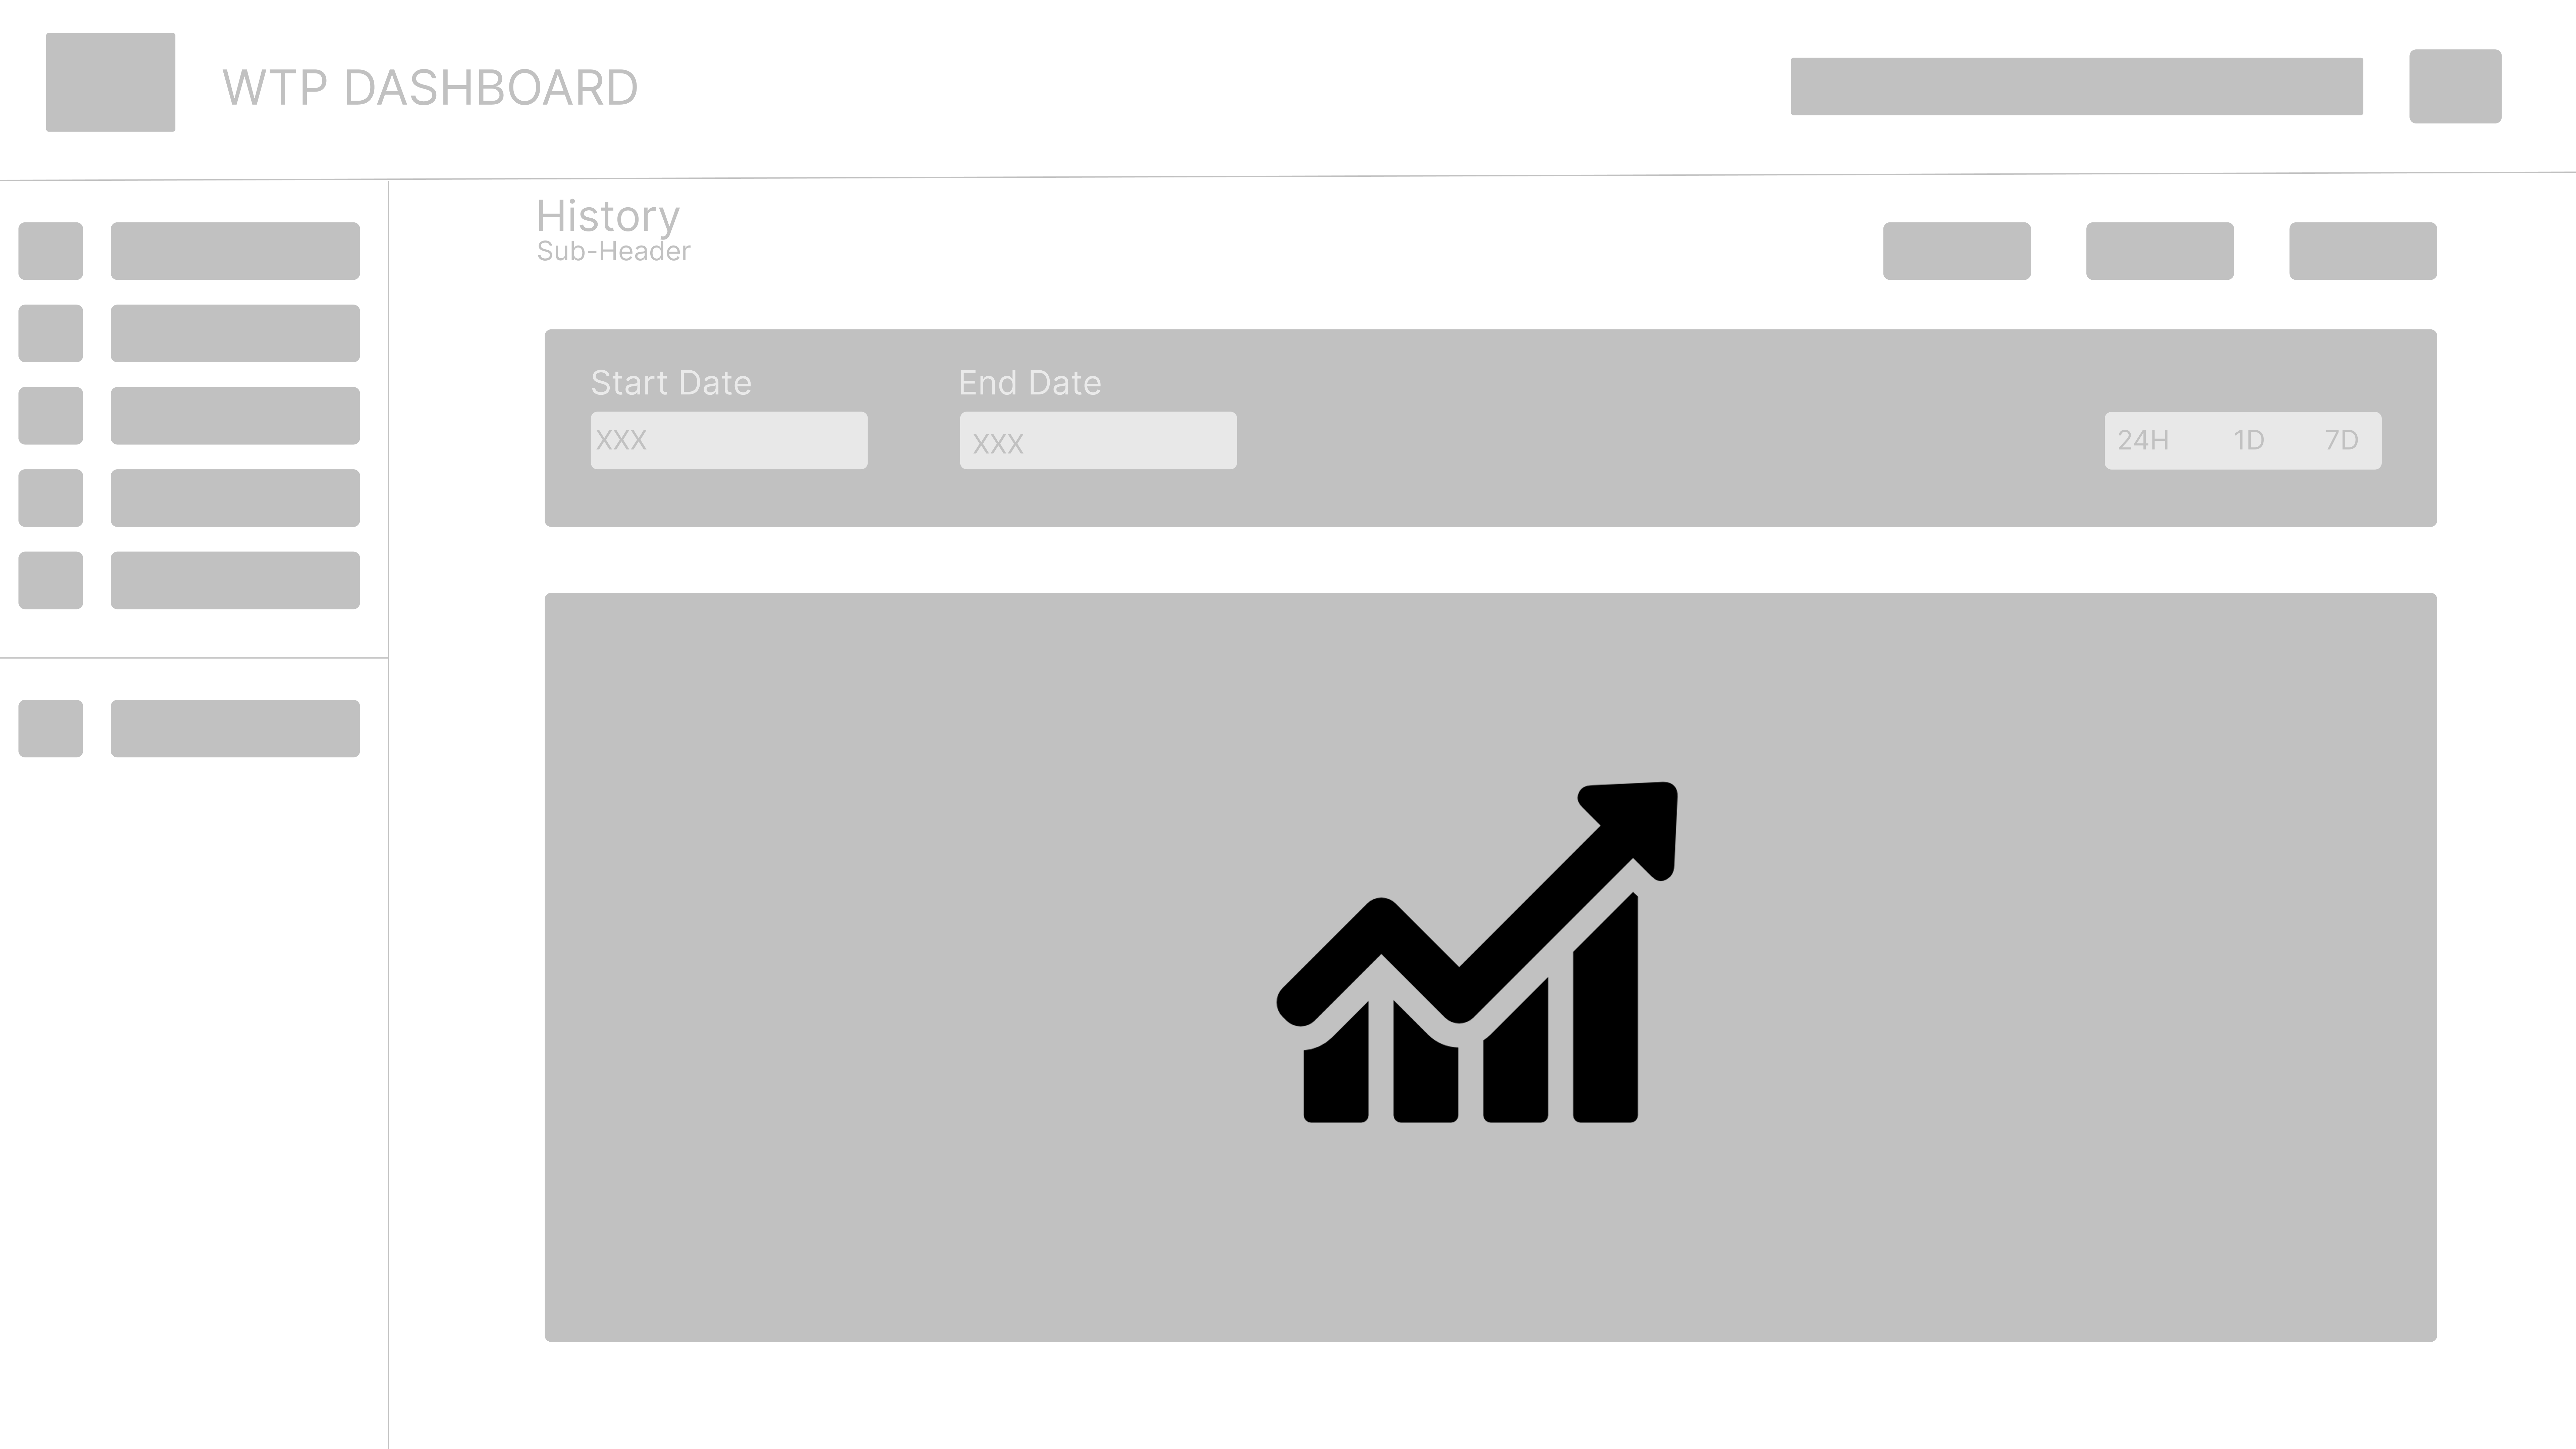
\includegraphics[width=\textwidth]{images/History-lowfi.png}
    \caption{Rancangan purwarupa \textit{low-fidelity} halaman riwayat sensor}
    \label{fig:ui-history}
\end{figure}

Tata letak halaman riwayat dipusatkan pada area kanvas grafik (\textit{chart canvas}) yang mendominasi sebagian 
besar layar untuk memperjelas visualisasi kurva data. Untuk mendukung interaktivitas, di bagian atas grafik 
disematkan komponen penyaring waktu (\textit{date picker}) yang memungkinkan operator menyesuaikan rentang kueri 
data (\textit{query parameter}) ke \textit{backend}. Sementara itu, di bagian bawah grafik disediakan representasi 
tabular (\textit{data table}) yang menyajikan titik-titik data grafik dalam bentuk angka eksak sehingga memudahkan 
proses validasi silang dan pembacaan metrik mentah.

\subsection{Antarmuka Halaman Log Alarm}
Halaman log alarm berfungsi sebagai pusat manajemen insiden. Oleh karena itu, antarmukanya dirancang agar operator dapat 
dengan cepat membaca detail anomali dan mengambil tindakan responsif. Rancangan purwarupa halaman alarm ditunjukkan pada 
Gambar~\ref{fig:ui-alarm}.

\begin{figure}[htbp]
    \centering
    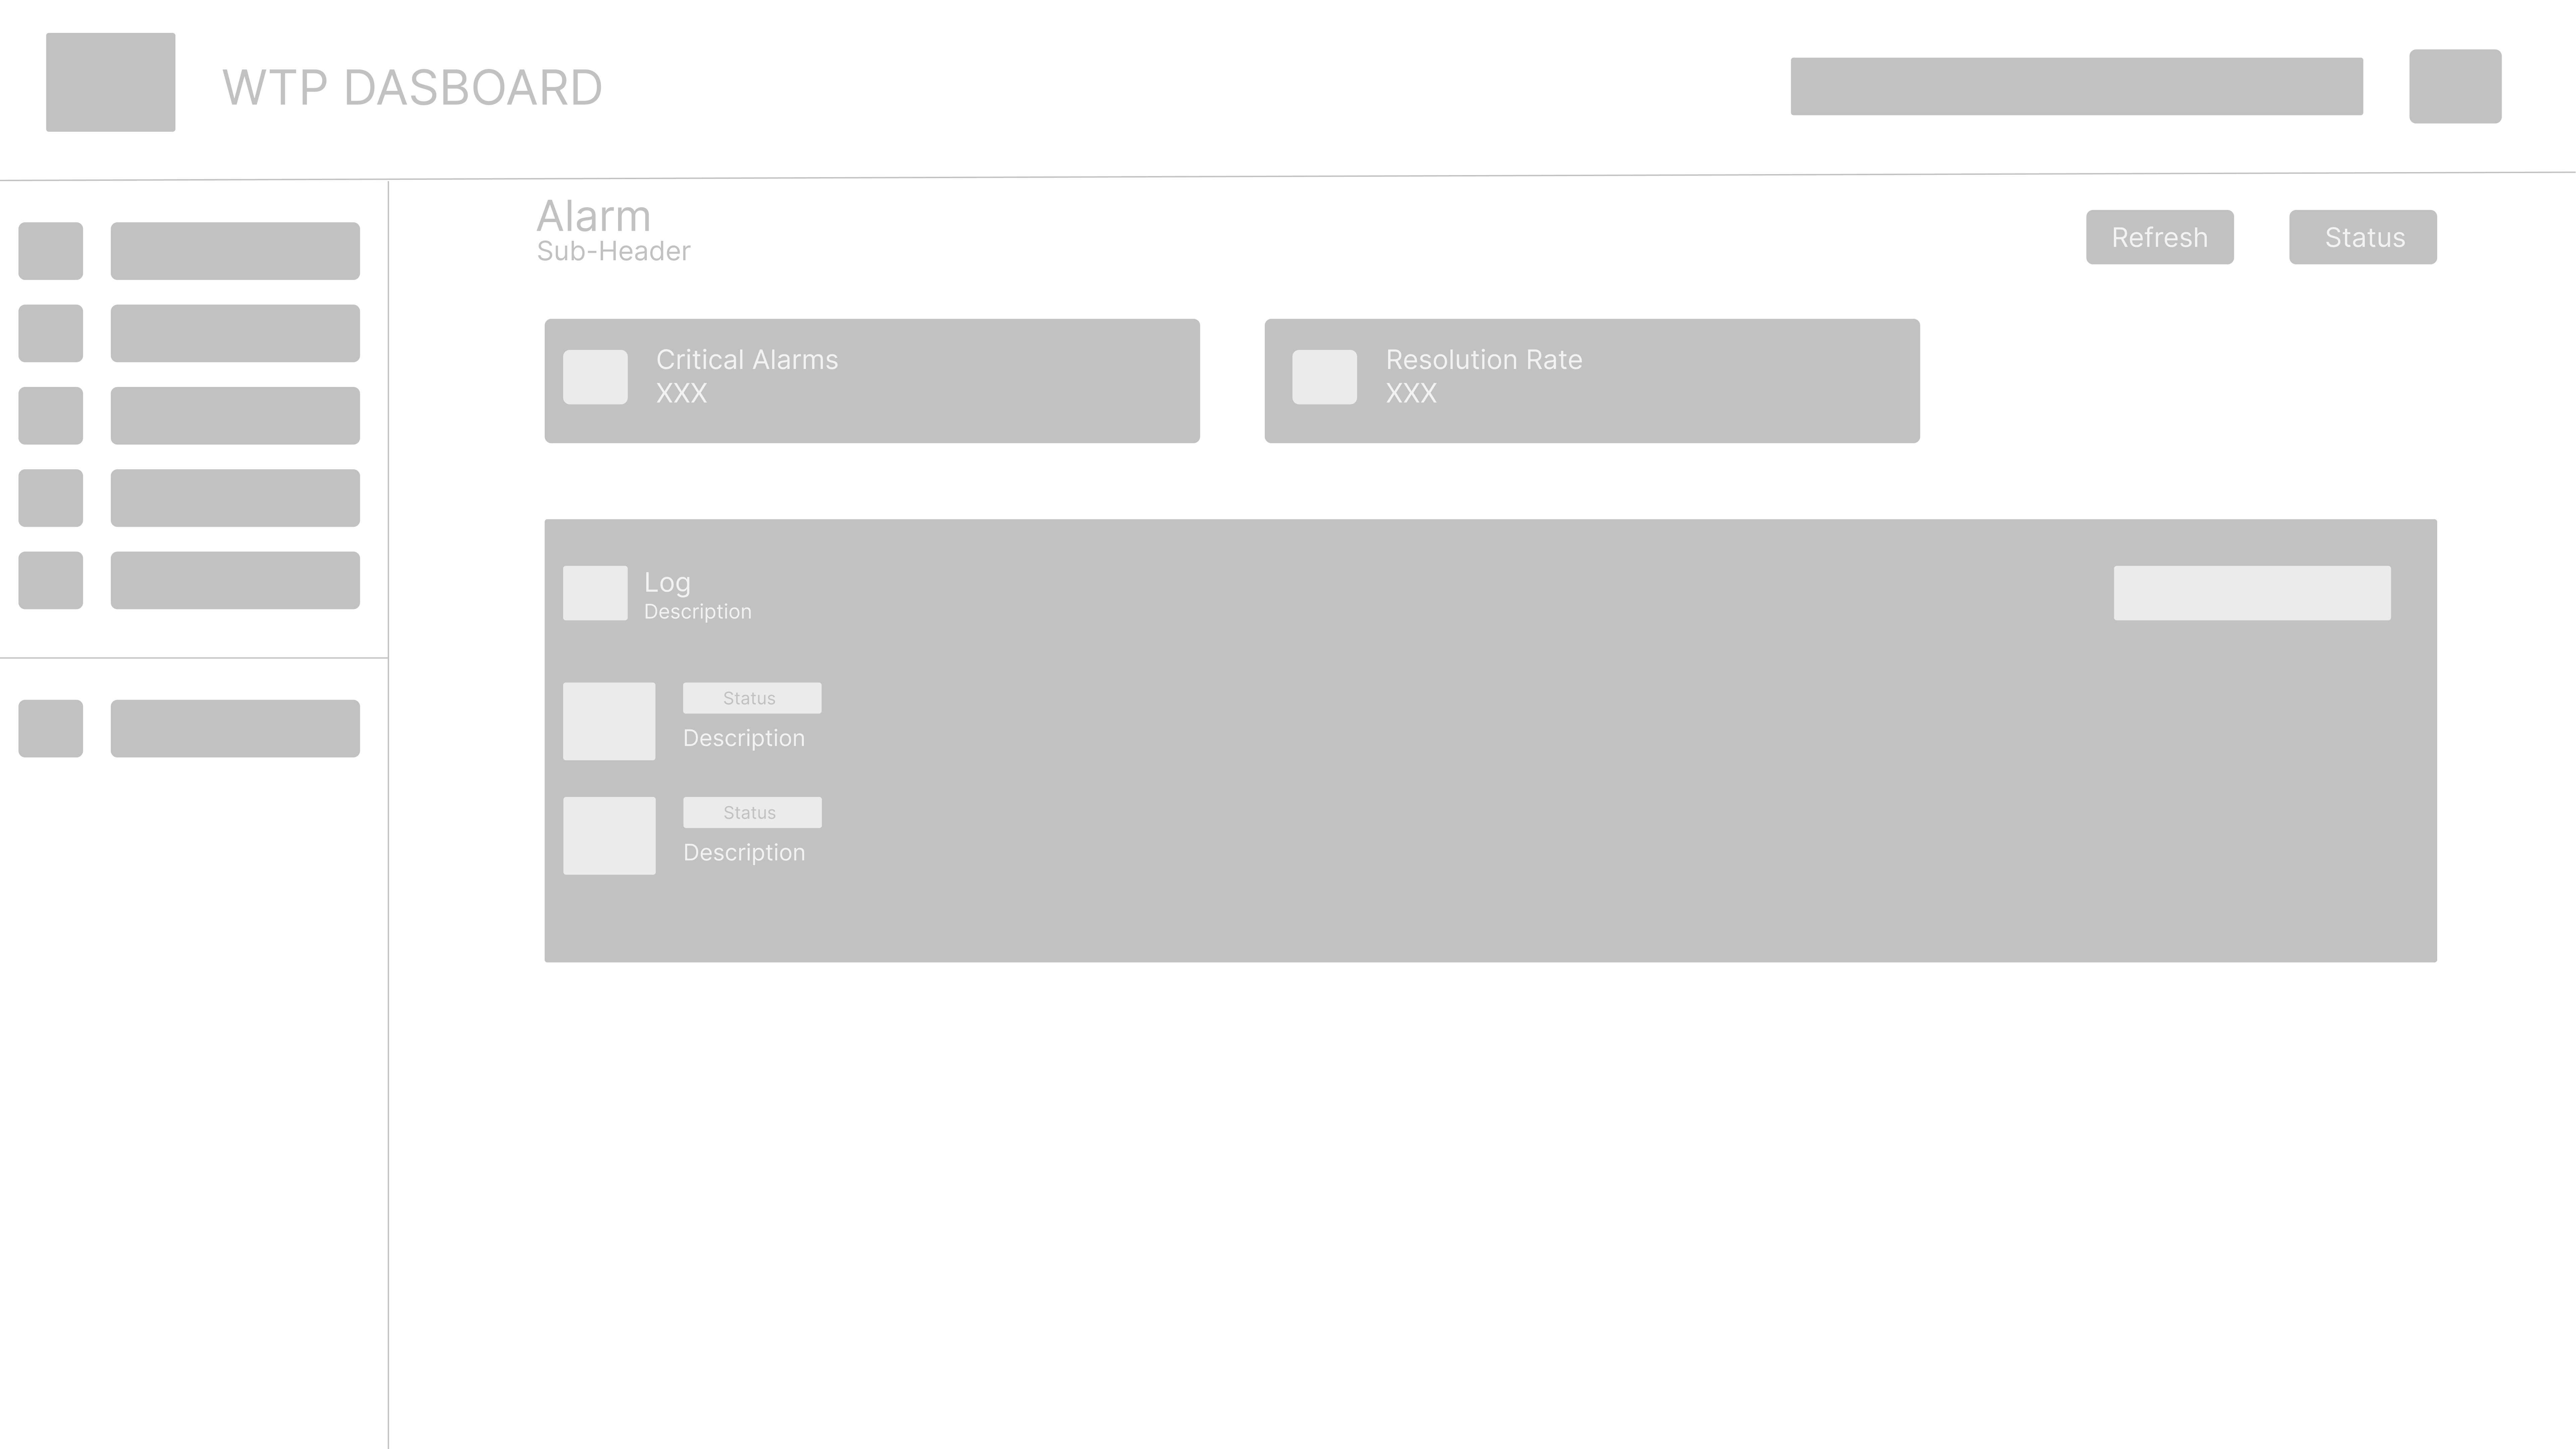
\includegraphics[width=\textwidth]{images/Alarm-lowfi.png}
    \caption{Rancangan purwarupa \textit{low-fidelity} halaman log alarm}
    \label{fig:ui-alarm}
\end{figure}

Seperti yang terlihat pada Gambar~\ref{fig:ui-alarm}, antarmuka halaman ini diorganisasikan menggunakan struktur 
daftar vertikal dinamis (\textit{dynamic vertical list}). Setiap baris di dalam daftar merepresentasikan satu kejadian 
(\textit{event}) unik. Komponen di dalam setiap baris mencakup lencana (\textit{badge}) sebagai indikator visual tingkat 
keparahan, deskripsi anomali, cap waktu (\textit{timestamp}) kejadian, serta sebuah tombol interaksi (\textit{action button}). 
Tombol tersebut diletakkan sejajar pada setiap baris untuk memfasilitasi operator dalam mengeksekusi tindakan pengakuan 
(\textit{acknowledge}) alarm secara cepat dan tepat sasaran tanpa harus berpindah halaman.

\subsection{Antarmuka Halaman Analitik Sensor}
Halaman analitik sensor dirancang untuk memberikan pemantauan terperinci terhadap masing-masing parameter 
kualitas air secara spesifik. Berbeda dengan halaman \textit{dashboard} utama yang merangkum status umum, 
halaman ini memfasilitasi analisis yang lebih mendalam untuk setiap instrumen pengukur. Rancangan purwarupa 
halaman analitik sensor ditunjukkan pada Gambar~\ref{fig:ui-sensor}.

\begin{figure}[htbp]
    \centering
    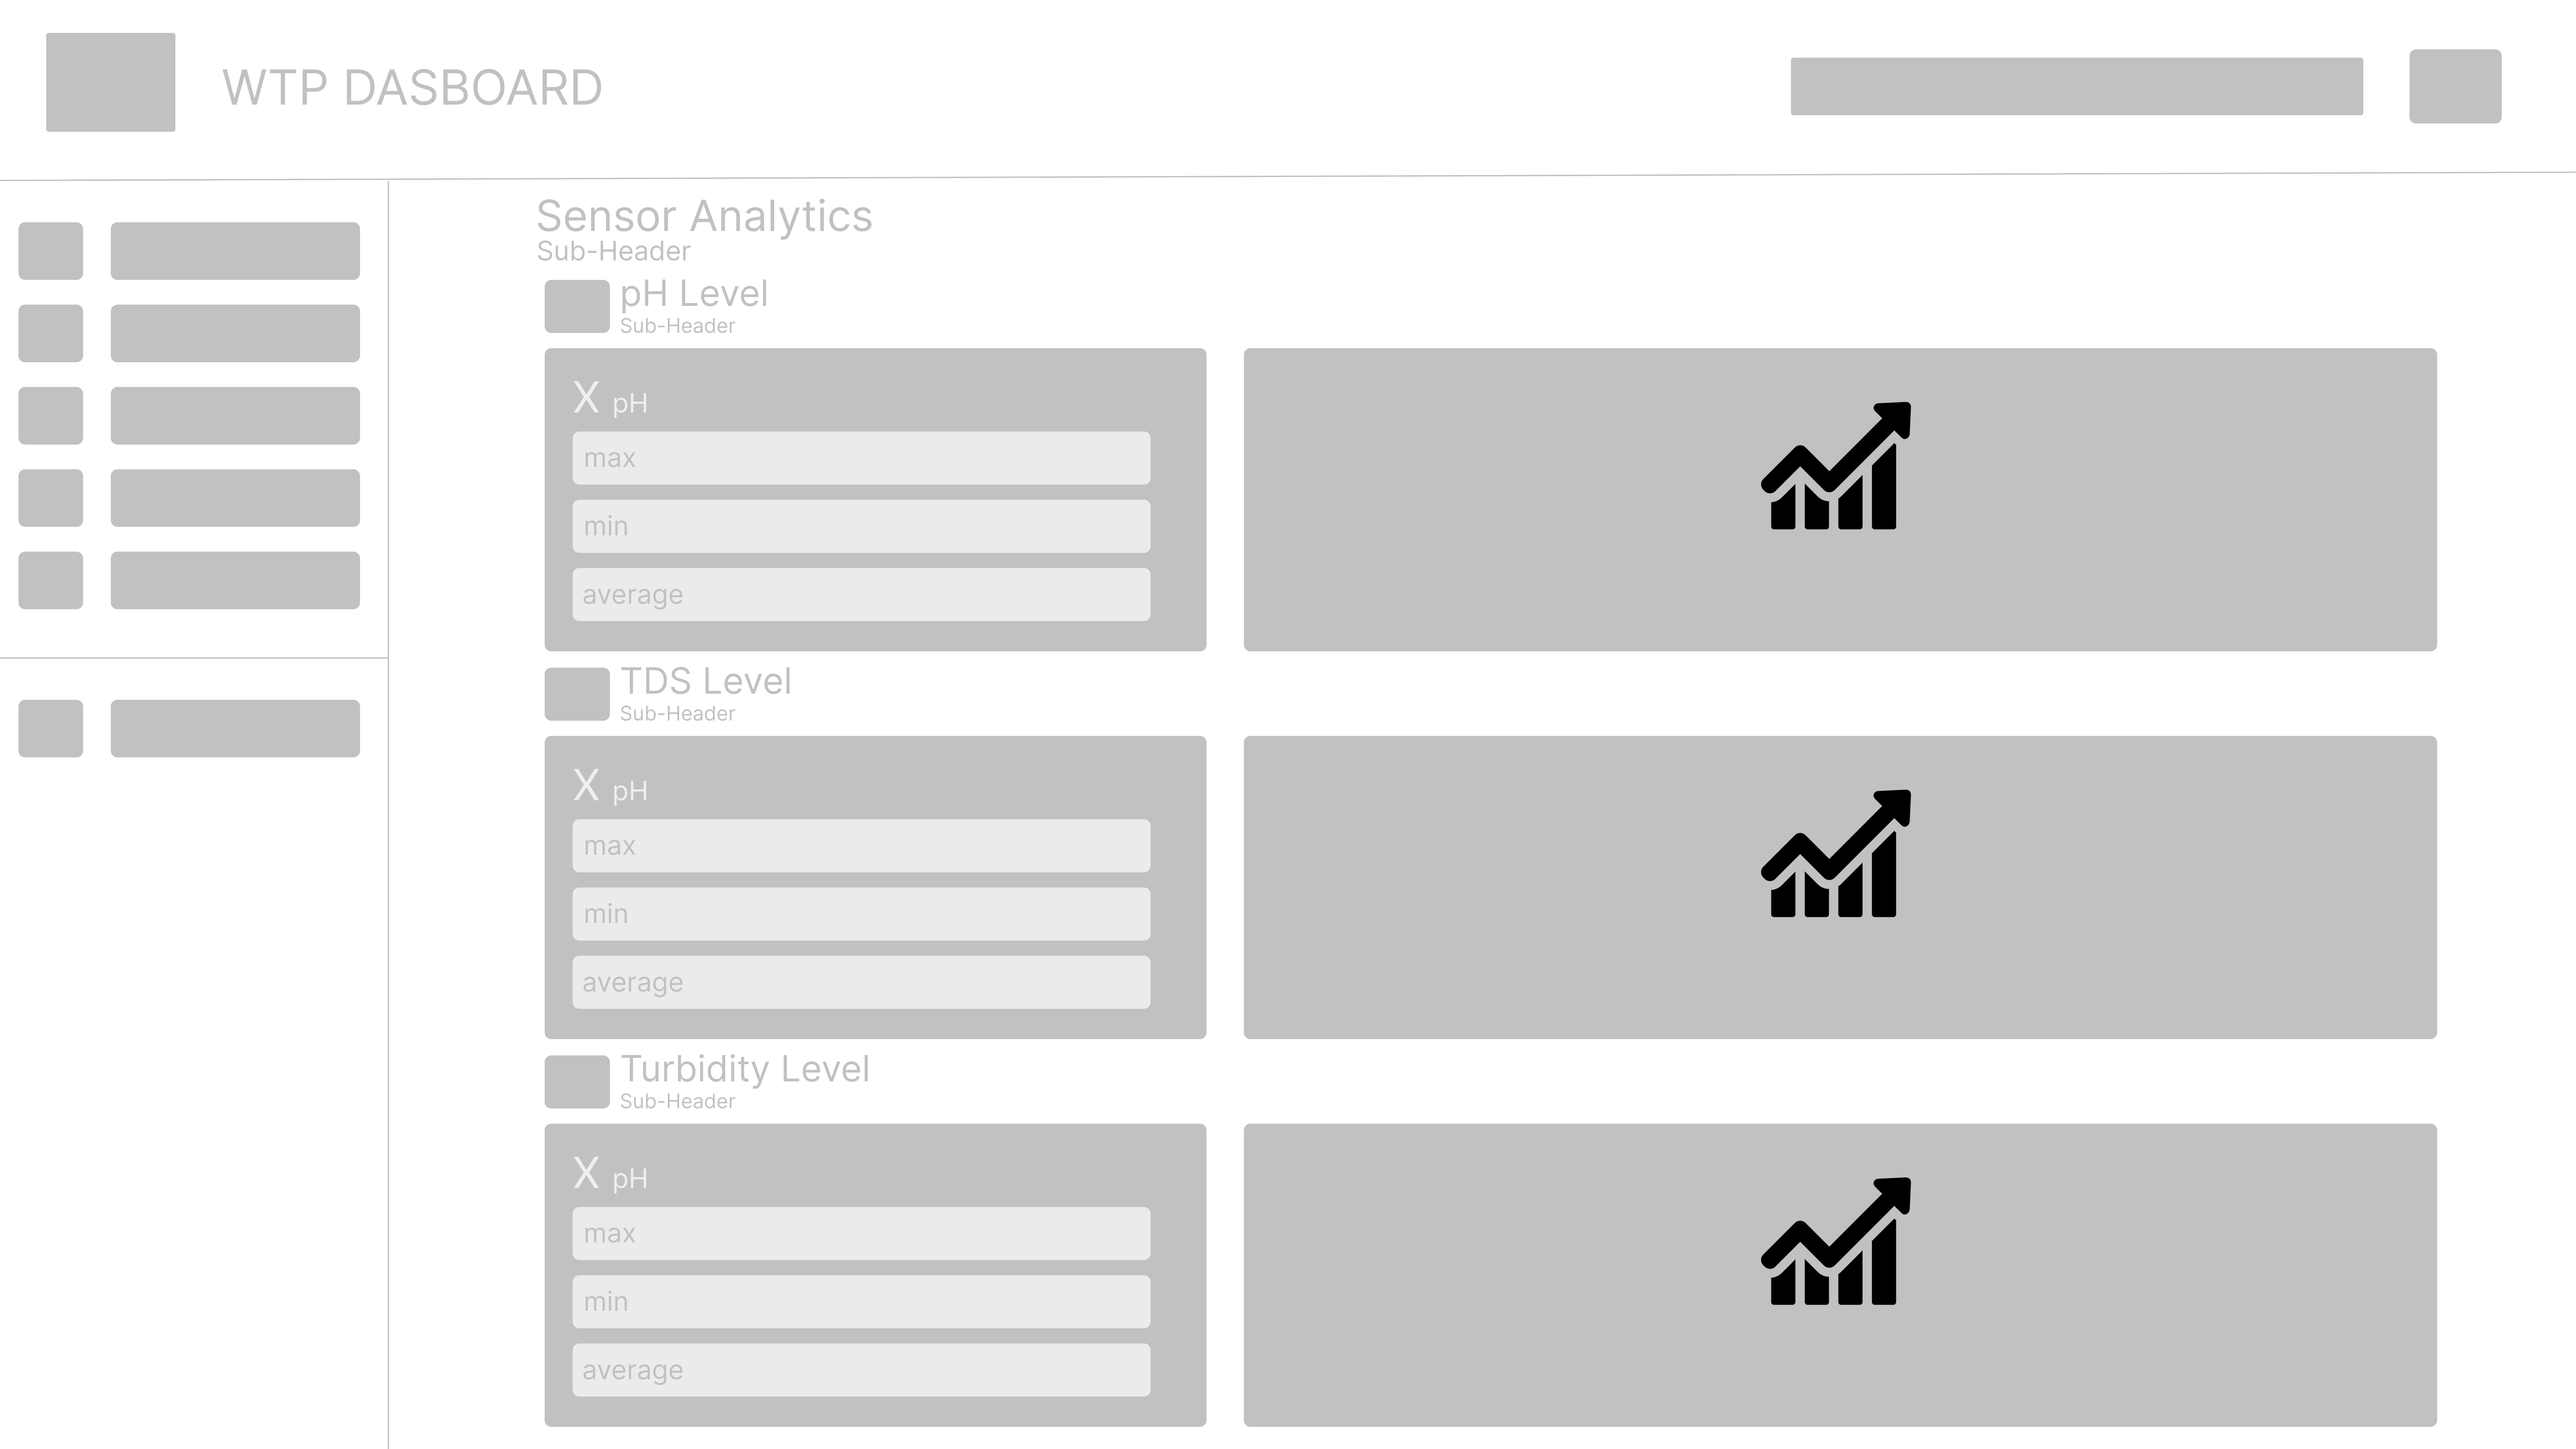
\includegraphics[width=\textwidth]{images/Sensor-lowfi.png}
    \caption{Rancangan purwarupa \textit{low-fidelity} halaman analitik sensor}
    \label{fig:ui-sensor}
\end{figure}

Berdasarkan Gambar~\ref{fig:ui-sensor}, antarmuka disusun secara vertikal berdasarkan kategori sensor utama, 
yaitu level pH, level TDS (\textit{Total Dissolved Solids}), dan level kekeruhan (\textit{Turbidity}). 
Pada setiap kategori, layar dibagi menjadi dua komponen fungsional utama yang diletakkan berdampingan (\textit{side-by-side}). 
Di sisi kiri, terdapat panel metrik yang menyajikan perhitungan statistik instan seperti nilai maksimum (\textit{max}), 
minimum (\textit{min}), dan rata-rata (\textit{average}). Di sisi kanan, ditempatkan kanvas grafik visualisasi tren data. 
Penyatuan representasi angka numerik dan grafik dalam satu blok pandang ini bertujuan untuk mempercepat proses kognitif 
operator dalam memahami perilaku fluktuasi air baku.

\subsection{Antarmuka Halaman Kendali Pompa}
Halaman kendali pompa dikhususkan sebagai antarmuka intervensi dan konfigurasi parameter operasional untuk setiap 
aktuator kimia atau pompa takaran (\textit{dosing pump}) yang ada pada sistem WTP. Desain halaman ini sangat mengutamakan 
kejelasan batas antarkomponen untuk menghindari kesalahan masukan (\textit{human error}) dari operator. Rancangan purwarupa 
halaman pompa dapat dilihat pada Gambar~\ref{fig:ui-pump}.

\begin{figure}[htbp]
    \centering
    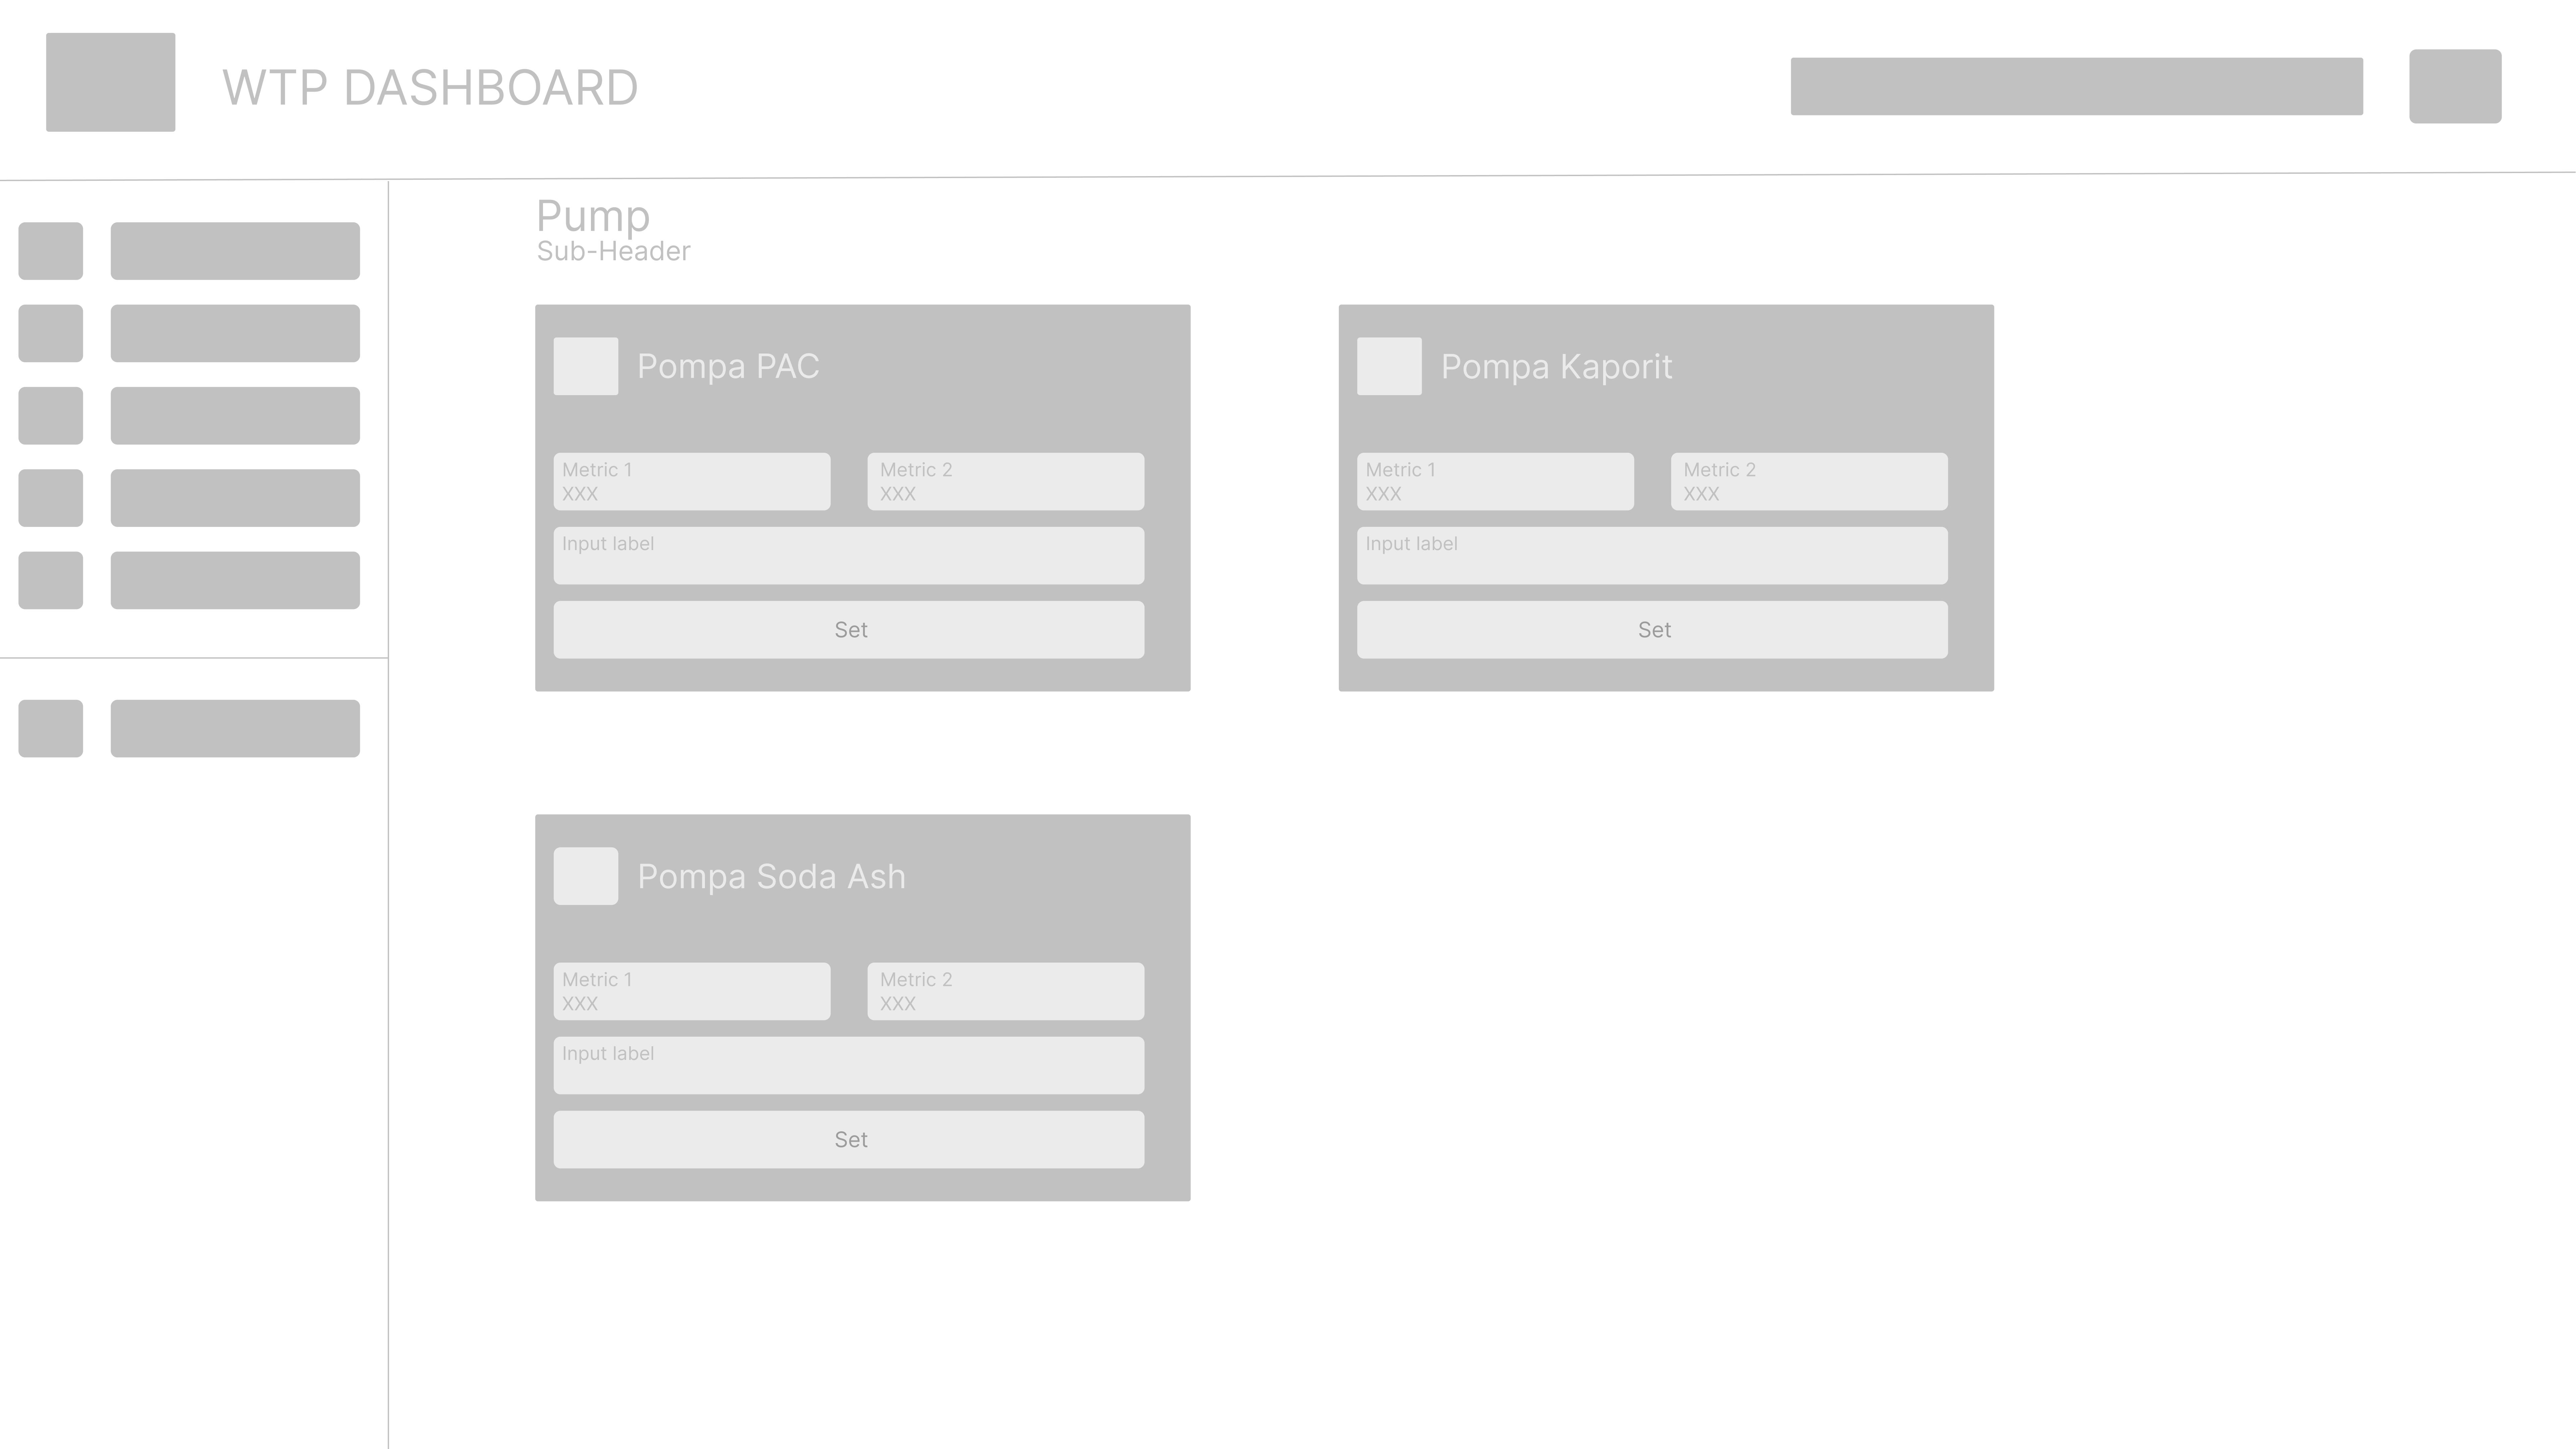
\includegraphics[width=\textwidth]{images/Pompa-lowfi.png}
    \caption{Rancangan purwarupa \textit{low-fidelity} halaman kendali pompa}
    \label{fig:ui-pump}
\end{figure}

Seperti yang diilustrasikan pada Gambar~\ref{fig:ui-pump}, halaman ini dipecah menjadi beberapa kartu komponen 
(\textit{card components}) yang terisolasi untuk masing-masing unit aktuator, di antaranya Pompa PAC, Pompa Kaporit, 
dan Pompa Soda Ash. Pemisahan antarkartu ini memberikan struktur logis yang tegas. Setiap kartu dilengkapi dengan kolom 
masukan (\textit{input fields}) untuk menetapkan variabel batas atau metrik penyesuaian dosis bahan kimia. Pada bagian 
bawah setiap kartu, disediakan sebuah tombol eksekusi aksi (tombol "Set") yang berfungsi untuk mengirimkan perintah 
titik acuan (\textit{set-point}) baru langsung ke backend melalui REST API. Tata letak ini dirancang agar proses kalibrasi dan 
kendali aktuator elektromekanis dapat dilakukan secara efisien, aman, dan tersentralisasi.

\section{Perancangan Aliran Data Telemetri}
Aplikasi \textit{dashboard} WTP menangani data telemetri yang bersumber dari \textit{backend} dan bersifat 
dinamis, yaitu dapat berubah nilainya sewaktu-waktu tanpa sepengetahuan \textit{frontend}. Oleh karena itu, 
diperlukan rancangan aliran data yang menjamin informasi yang disajikan kepada operator tetap konsisten dengan 
kondisi terbaru pada \textit{backend}, sejalan dengan prinsip keterandalan informasi yang dijabarkan pada 
Subbab~\ref{sec:tahapan-perancangan}.

\subsection{Karakteristik Data yang Dikelola}
Data yang dialirkan dari \textit{backend} mencakup data telemetri terkini, pembacaan riwayat historis, log 
kejadian alarm, dan nilai \textit{offset} dosis bahan kimia. Karakteristik utama dari seluruh data tersebut 
adalah sifatnya yang asinkron, sumber kebenarannya (\textit{source of truth}) berada di \textit{backend}, dan 
berpotensi menjadi usang (\textit{stale}) apabila tidak disinkronisasi secara berkala.

\subsection{Mekanisme Aliran Data}
Aliran data dirancang melalui tiga mekanisme yang saling berkaitan.

\begin{enumerate}
    \item \textbf{Pengambilan dan penyimpanan sementara (\textit{fetching} dan \textit{caching}).} Data yang 
    diminta dari \textit{backend} disimpan sementara setelah diterima, sehingga permintaan berikutnya terhadap 
    data yang sama tidak perlu selalu menempuh jaringan, selama data tersebut belum dinyatakan usang.
    
    \item \textbf{Pembaruan berkala (\textit{polling}).} Data telemetri seperti pH dan kekeruhan memerlukan 
    penyajian yang mendekati kondisi terkini. Oleh karena itu, aliran data dirancang untuk menarik ulang data 
    dari \textit{backend} secara berkala dengan interval lima detik, tanpa memerlukan penyegaran halaman oleh 
    operator. Skenario ini diilustrasikan pada Gambar~\ref{fig:sequence-state}.
    
    \item \textbf{Invalidasi setelah mutasi.} Untuk interaksi yang mengubah data pada \textit{backend}, seperti 
    pengiriman \textit{offset} dosis, aliran data dirancang agar begitu perubahan berhasil dikonfirmasi oleh 
    \textit{backend}, seluruh data terkait yang tersimpan sementara pada \textit{frontend} dinyatakan usang dan 
    ditarik ulang secara paksa. Mekanisme ini mencegah antarmuka menampilkan nilai lama setelah operator 
    melakukan perubahan, sebagaimana turut diilustrasikan pada Gambar~\ref{fig:sequence-state}.
\end{enumerate}

\begin{figure}[t]
    \centering
    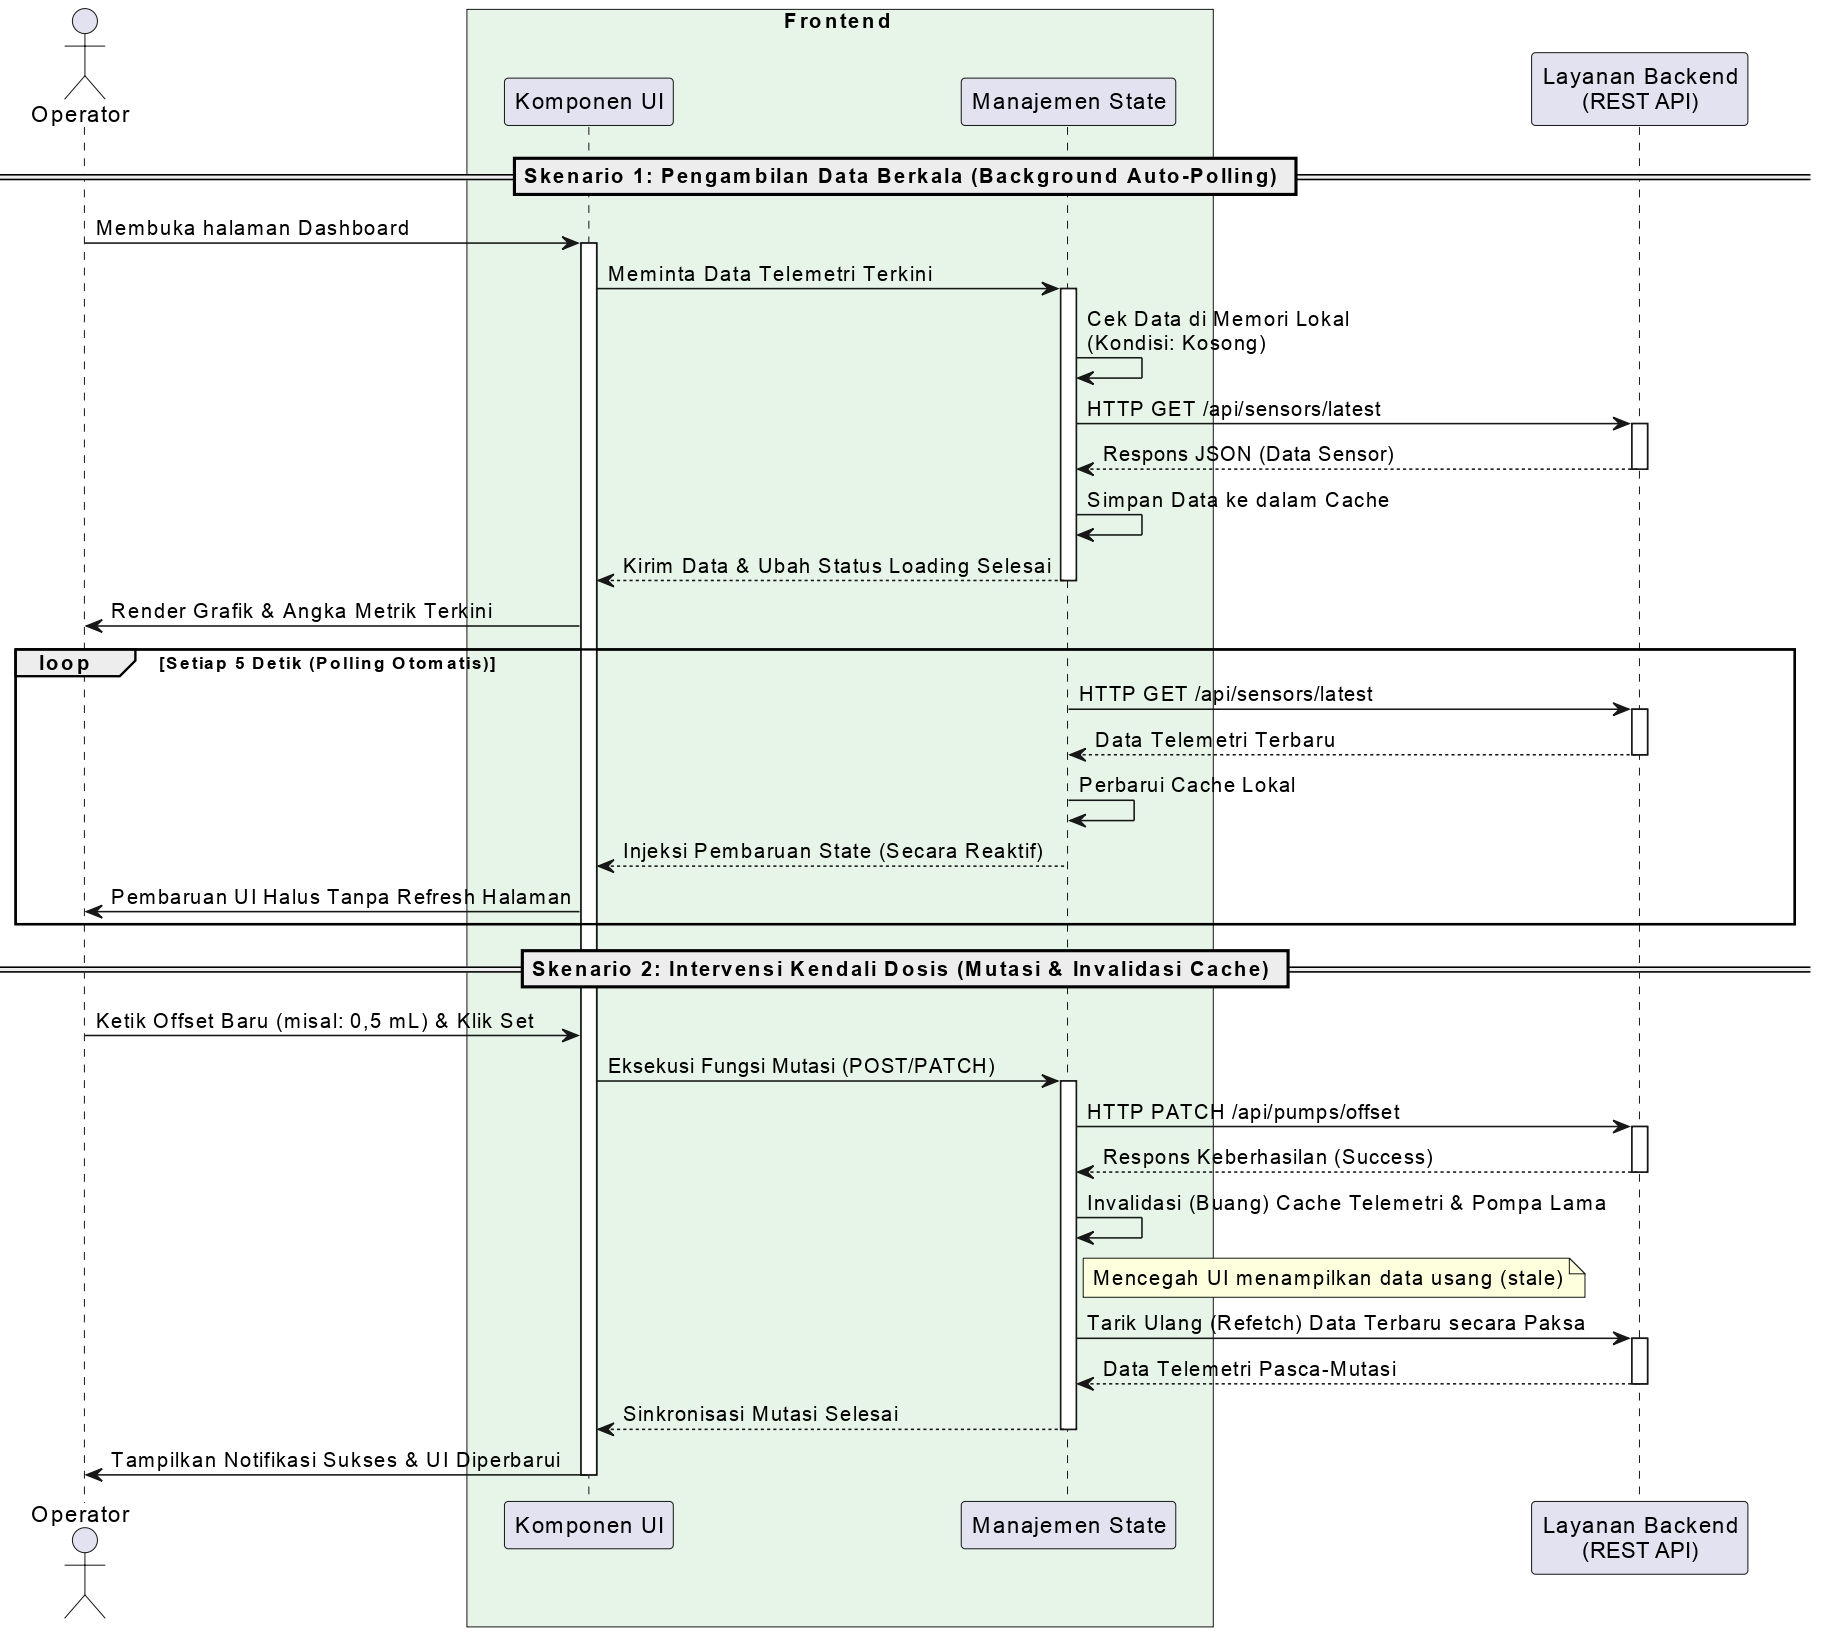
\includegraphics[width=\textwidth]{images/sequence-state.jpg}
    \caption{Diagram sekuens aliran data pada pembaruan berkala dan invalidasi pasca-mutasi}
    \label{fig:sequence-state}
\end{figure}

Ketiga mekanisme tersebut menjadikan operator selalu mendapatkan data yang konsisten dengan kondisi 
\textit{backend} terkini, baik pada kondisi pemantauan pasif (\textit{polling}) maupun setelah operator 
melakukan intervensi aktif (mutasi).

\section{Perancangan Kontrak API}
Perancangan kontrak API (\textit{API Contracts}) berfungsi sebagai dokumen kesepakatan spesifikasi komunikasi antara 
layanan \textit{frontend} dan \textit{backend}. Kontrak ini mendefinisikan secara presisi struktur data yang akan dikirim 
(\textit{request payload}) dan struktur data yang akan diterima (\textit{response payload}). 

Pada pengembangan sistem \textit{dashboard} WTP ini, spesifikasi kontrak diimplementasikan dan ditegakkan 
secara ketat menggunakan definisi antarmuka (\textit{interface}) berbasis pengetikan statis (\textit{static typing}). Pendekatan ini memberikan jaminan keamanan 
tipe data (\textit{type safety}) pada saat kompilasisehingga meminimalisasi potensi galat (\textit{runtime error}) 
yang diakibatkan oleh atribut data yang hilang atau ketidaksesuaian struktur objek data dari \textit{backend}.

Secara arsitektural, sistem ini memanfaatkan berbagai \textit{endpoint} yang dikelompokkan berdasarkan modul 
fungsionalnya, mulai dari autentikasi hingga kendali aktuator. Ringkasan seluruh \textit{endpoint} yang digunakan 
pada sistem ini dapat dilihat pada Tabel~\ref{tab:api-summary}.

\begin{table}[t]
    \centering
    \caption{Ringkasan Kontrak API Sistem WTP}
    \label{tab:api-summary}
    \renewcommand{\arraystretch}{1.2}
    \begin{tabular}{|p{3cm}|p{4.5cm}|c|p{5cm}|}
        \hline
        \textbf{Modul} & \textbf{Endpoint} & \textbf{Metode} & \textbf{Fungsi Utama} \\
        \hline
        \multirow{5}{*}{Autentikasi} 
        & /api/auth/login & POST & Autentikasi kredensial lokal \\
        & /api/auth/google & POST & Autentikasi melalui penyedia identitas pihak ketiga (OAuth 2.0) \\
        & /api/auth/logout & POST & Mengakhiri sesi pengguna \\
        & /api/auth/refresh & POST & Memperbarui token akses \\
        & /api/auth/me & GET & Mengambil profil pengguna aktif \\
        \hline
        \multirow{4}{*}{Telemetri \& Sensor} 
        & /api/sensors/latest & GET & Mengambil data sensor terkini \\
        & /api/history & GET & Mengambil riwayat data historis \\
        & /api/dashboard/summary & GET & Metrik agregasi untuk \textit{dashboard} \\
        & /api/export & GET & Mengunduh laporan data kualitas air \\
        \hline
        \multirow{2}{*}{Manajemen Alarm} 
        & /api/alarms & GET & Mengambil daftar log anomali \\
        & /api/alarms/:id & PATCH & Mengubah status (\textit{acknowledge}) alarm \\
        \hline
        \multirow{4}{*}{Kendali Pompa} 
        & /api/pumps & GET & Mengambil status seluruh pompa \\
        & /api/pumps/offsets & GET & Mengambil konfigurasi dosis saat ini \\
        & /api/pumps/:pumpId/offset & PATCH & Memperbarui nilai \textit{offset} dosis \\
        & /api/pumps/:pumpId/status & PATCH & Menghidupkan/mematikan pompa spesifik \\
        \hline
        \multirow{2}{*}{Notifikasi} 
        & /api/push/subscribe & POST & Mendaftarkan perangkat untuk \textit{push notification} \\
        & /api/push/unsubscribe & DELETE & Mencabut akses notifikasi perangkat \\
        \hline
    \end{tabular}
\end{table}

Meskipun sistem mengimplementasikan seluruh \textit{endpoint} pada Tabel~\ref{tab:api-summary}, 
penjabaran kontrak struktur data secara mendetail difokuskan pada tiga \textit{endpoint} inti yang 
merepresentasikan aliran data kritikal pada operasional WTP, yaitu akuisisi telemetri terkini, pengambilan 
data historis, dan pengiriman perintah intervensi dosis.

\subsection{Endpoint Telemetri Terkini (\textit{Latest Telemetry})}
\textit{Endpoint} ini menggunakan metode HTTP GET untuk melayani kebutuhan komponen \textit{dashboard} utama. 
Struktur datanya dirancang datar (\textit{flat object}) untuk meminimalkan waktu pemrosesan (\textit{parsing}) 
di sisi peramban sehingga metrik waktu nyata seperti pH, kekeruhan, dan status operasional pompa dapat langsung 
diekstrak dan dirender oleh komponen antarmuka.

Kontrak lengkap struktur data dan contoh objek respons untuk telemetri terkini disertakan pada Lampiran~\ref{lst:telemetry-latest}.

\subsection{Endpoint Riwayat Historis (\textit{Historical Data})}
Untuk mendukung visualisasi grafik tren, \textit{frontend} membutuhkan kumpulan data berdasarkan rentang 
waktu spesifik. Oleh karena itu, \textit{endpoint} ini (menggunakan metode GET) mengembalikan respons berupa 
susunan (\textit{array of objects}). Setiap objek di dalam susunan tersebut mewakili satu titik data (\textit{data point}) 
yang terikat dengan cap waktu (\textit{timestamp}) masing-masing.

Kontrak lengkap struktur data dan contoh objek respons untuk riwayat sensor disertakan pada Lampiran~\ref{lst:telemetry-history}.

\subsection{Endpoint Intervensi Dosis (\textit{Dose Offset Command})}
Berbeda dengan dua \textit{endpoint} sebelumnya yang bersifat pasif (hanya mengambil data), \textit{endpoint} 
ini bersifat aktif. \textit{Frontend} mengirimkan data (\textit{request body}) ke \textit{backend} menggunakan 
metode HTTP POST atau PUT untuk mengubah variabel kontrol di lapangan. Selain mengirimkan nilai \textit{offset}, 
kontrak ini mewajibkan pengiriman identitas operator (\texttt{updatedBy}) untuk keperluan audit keamanan dan 
pelacakan riwayat intervensi.

Kontrak lengkap permintaan (\textit{request}) dan respons untuk \textit{offset} dosis disertakan pada Lampiran~\ref{lst:dose-offset}.

Dengan disepakatinya ketiga jenis kontrak pertukaran data tersebut, integrasi sistem menjadi lebih terarah. \textit{Frontend} 
dapat mendasarkan seluruh proses pengambilan data, perenderan komponen antarmuka, hingga transmisi parameter 
\textit{offset} dosis pada struktur pengetikan statis yang telah didefinisikan secara baku.